\chapter{Monolithic silicon pixel detectors}\label{ch:2}

The first particle detection experiments at accelerator were usually set-up following the fixed target approach meaning that the beam of incoming particles would be shot on a stationary target. The detector for these particular experiments would then cover a rather small region in space and in momentum to detect single particles produced in the interaction. Simply scanning as the function of angle and momentum acceptances, the number of particles with a counter, one could reconstruct the kinematics of the particles. Concurrently, since the 1950s, other detector layouts like bubble chambers allowed physicist to register at a larger scale the full interaction of the particles involved, but the analysis work of the single exposures turns the detecting method very laborious. 

For quite some time, optical recording by photographic exposures remained the only choice to capture complex particle interaction within large detecting volumes. Although, since the 1960s, the transition towards detectors profiting from fully electronic readout started in parallel to the development of highly integrated circuits. This advancement in technology brought a solution to the arduous readout of bubble chambers but in environments such as the LHC were high radiation levels are encountered, the rates limitations from technologies such as MultiWire Proportional Chambers (MWPCs) forced by the large collections electrodes slowly became a problem too. 

In modern particle physics, the fixed target approach is often disfavoured to the head on or collider type of experiments in which bunches of particles are both accelerated and collide at the core of a detector. The goal is then to cover as much as possible of solid angle around the interaction point, detecting, identifying and kinematically reconstructing all the particles produced in the scattering process. If one had to give a general description of the detectors designed for collider experiments, it would generally be constructed in a cylindrical arrangement around the accelerator's beam pipe. It would notably require in its inner parts a vertex detector and tracking detectors respectively for identification of secondary vertices from the initial reaction vertex and reconstruction of tracks leading to momentum reconstruction and in some cases also particle identification\ \cite{detectors}. 

The high event rates combined with high spatial resolution required and low amount of material needed in the innermost layers of the detectors put in evidence semiconductors detectors as the preferred solution for the future experiments. This direction was even more praised by the fast development of microelectronics technics and their intrinsic properties such as densities and low energy threshold required for ionisation. Recent studies in this field has also proven this technology to be providing excellent timing performances which, as discussed previously, will be one of the key requirement for future particle tracking systems at collider experiments. In the following chapter a description of semiconductors devices for particle detection will be provided, and some more advanced concepts will be discussed as part of the focus of this work. 

	\section{Fundamentals of semiconductors}\label{sec:2.1}
	Semiconductors are classified together with insulators and conductors as one of the three type of solid material. Their electric resistivity (or equivalently electrical conductivity) is found in between the range of insulators ($10^8$ \SI{}{\ohm\centi\meter} and above) and the one of conductors ($10^-3$ \SI{}{\ohm\centi\meter} and below). Different types of pure semiconductors or compound will have different resistivities. Silicon (Si) is the most widely used semiconductor both for the detection material and readout chip of the present detectors, thanks to its large abundance on Earth but also to its intrinsic properties which will be discussed later.

		\subsection{Intrinsic and doped semiconductors}\label{subsec:2.1.1}
		The different properties of semiconductors are defined by the arrangement of the atoms within their crystalline structure. Silicon crystals are arranged in a diamond lattice so that each Si atom is covalently bonded to four nearest neighbors arranged at the corners of a tetrahedron\ \cite{SolidState}. From this specific structure, the diverse crystal planes are usually used for slicing the crystals to obtain a different arrangement and density of atoms and hence different properties for various applications using the same semiconductor material\ \cite{Si_Crystals_planes}. 

		The compact and periodic arrangement of atoms in the lattice give rise to a separation so thin in the energy levels of individual atoms due to the influence of many neighbouring atoms that one has to consider energy bands rather than single energy levels. The energy bands are separated by a so-called band-gap and the electrical conduction properties are defined by the two highest energy bands respectively the valence band and the conduction band. The conduction properties really depend on the energy difference between the bands as the energy levels within the bands themselves are so dense that transitions to unoccupied levels can seamlessly be done.
		\begin{figure*}[h]
		\begin{minipage}{0.49\linewidth}
		For insulators, the valence band is completely filled due to the very strong bonds between the neighbouring atoms, the conduction band is then empty, and the band gap is very large, about \SI{9}{\electronvolt} at room temperature. It is then very unlikely that by thermal excitation, an electron can rise from the valence band to the conduction band, current can't flow in insulators. In semiconductors, the neighbouring atoms are less bonded to each other, this leads to a smaller band gap energy, for Silicon it is about \SI{1.12}{\electronvolt} at room temperature. By thermal excitation of the action on an electric field, an electron can be moved to the conduction band leaving behind a hole in the valence band, current can then flow. 

		\end{minipage}\hfill
		\begin{minipage}{0.49\linewidth}
		\centering
		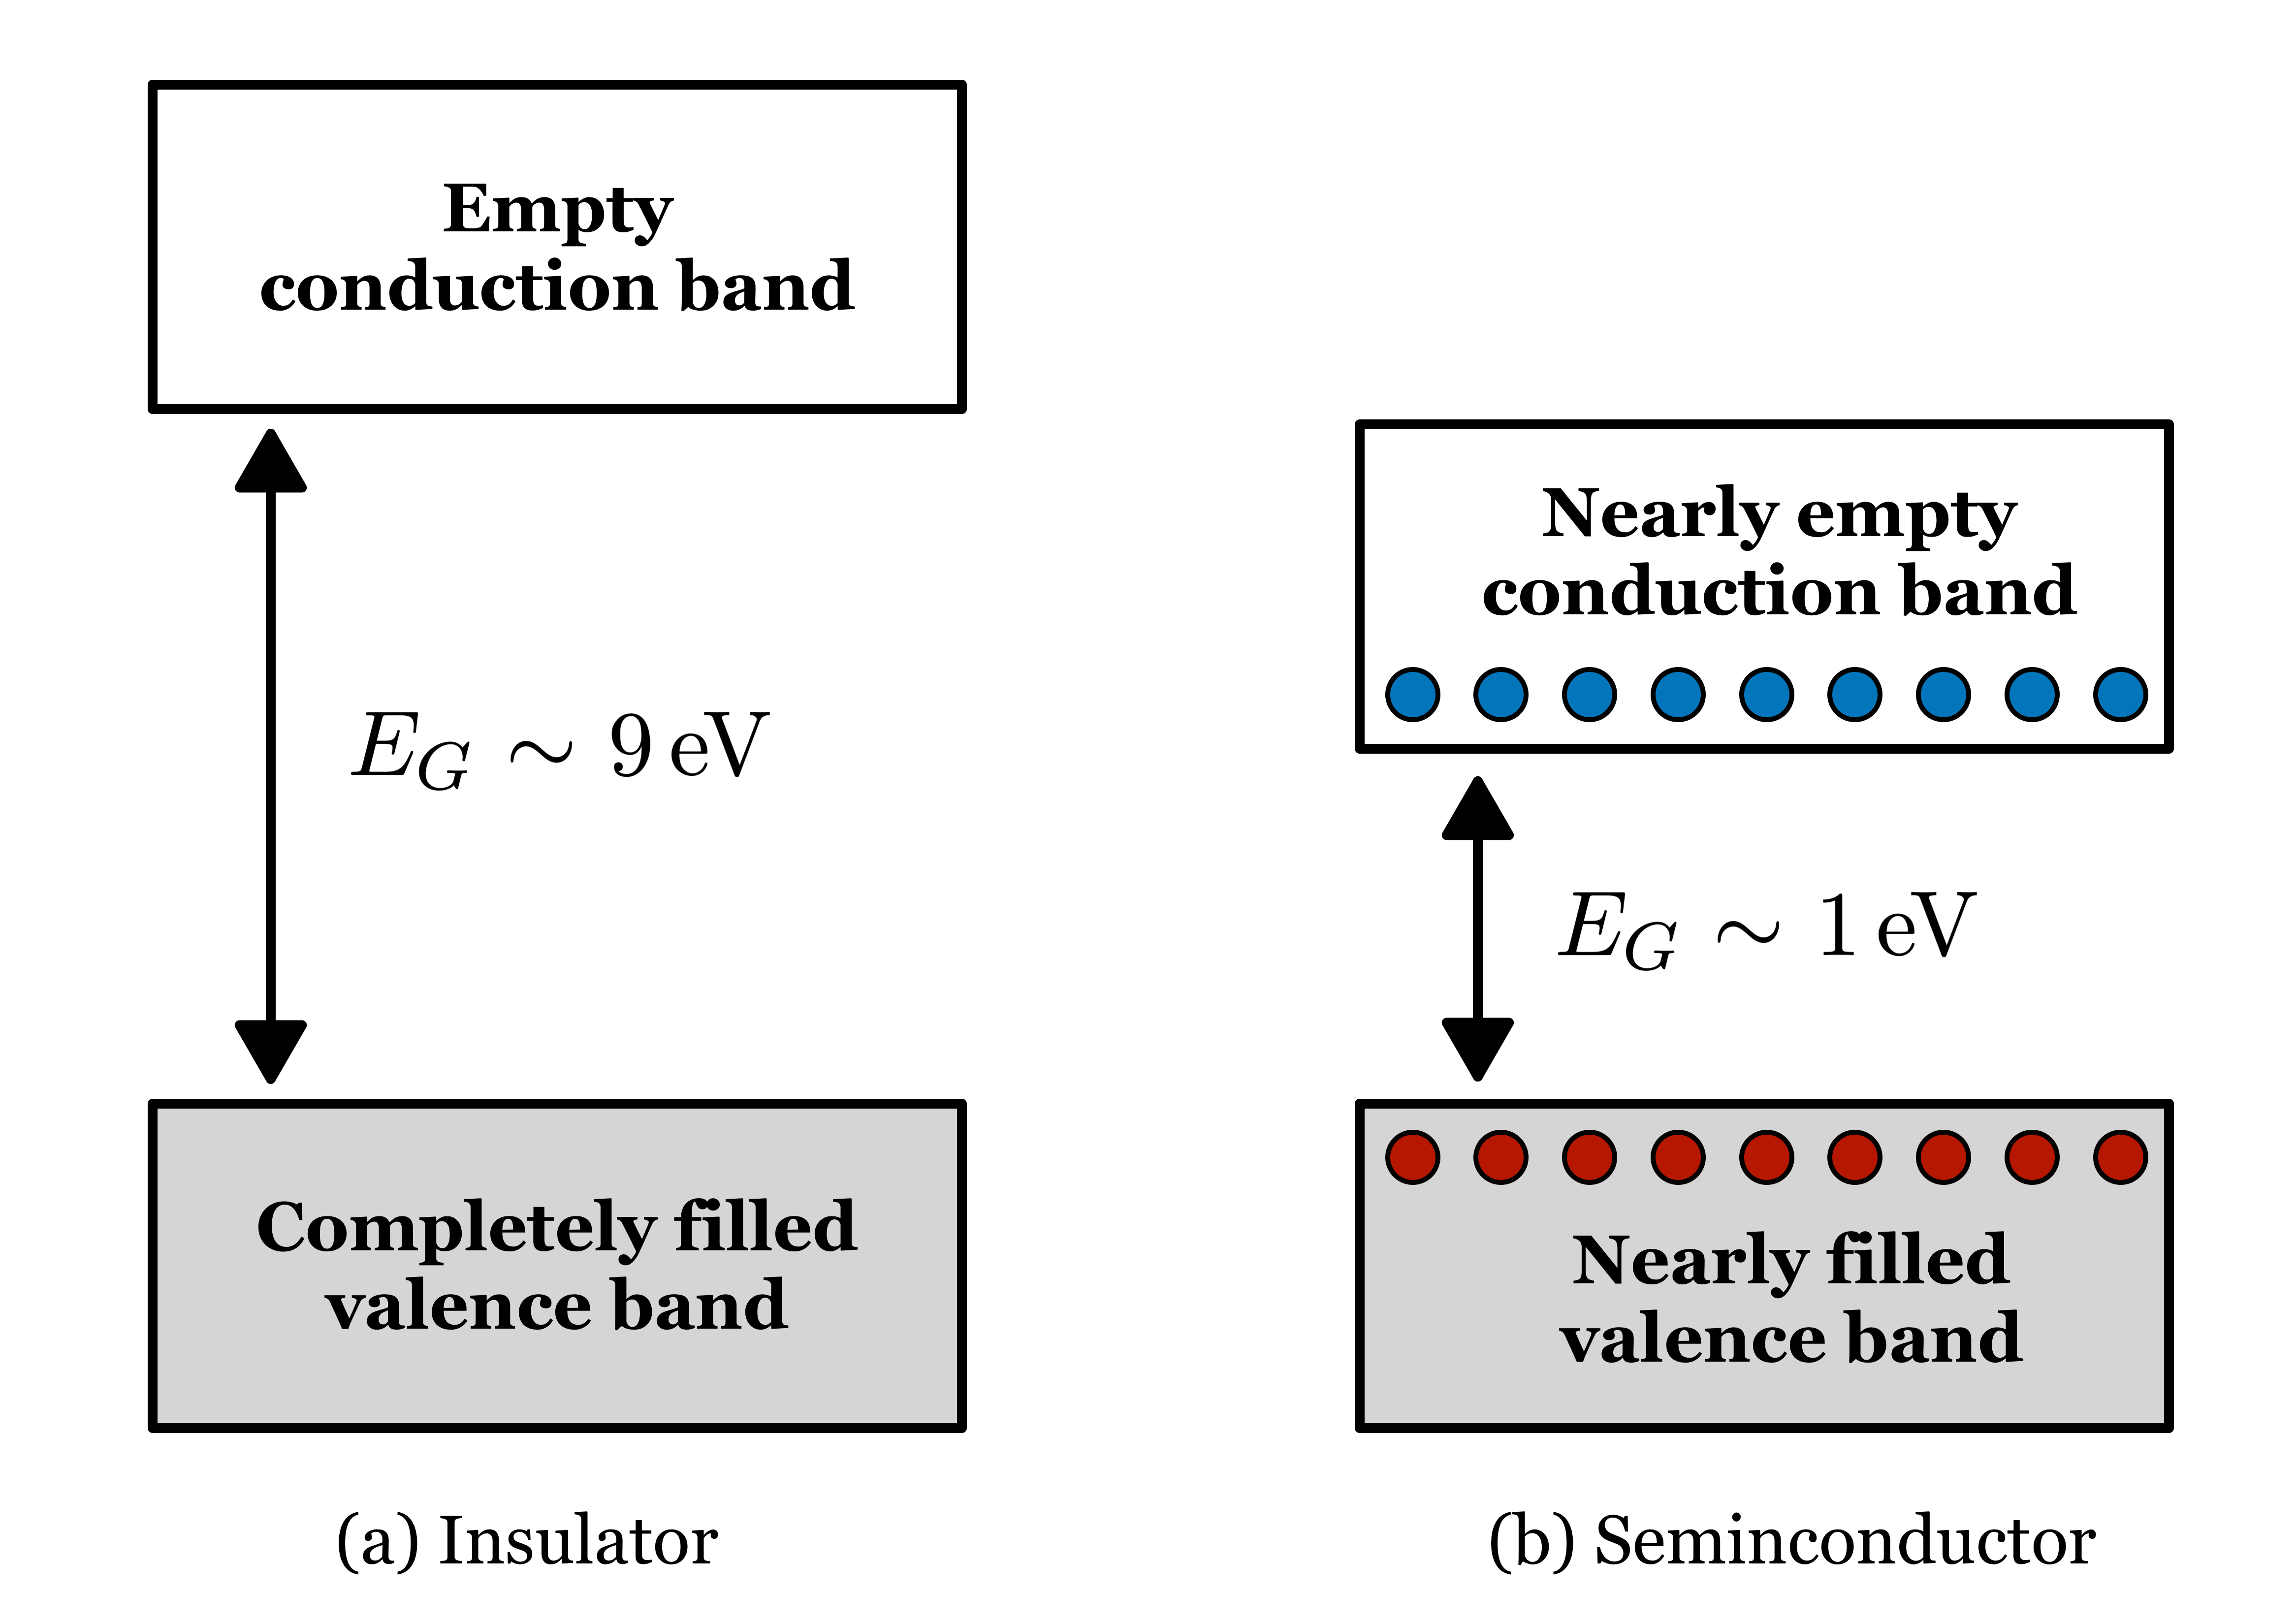
\includegraphics[width=1.0\linewidth]{files/energybands_insu_semi}
		\caption{Schematic view of the separation between valence and conduction bands for a) an insulator and b) a semiconductor.}
		\label{ }
		\end{minipage}
		\end{figure*}

		The gap in energy separating the bands can be influenced by temperature or pressure as it is directly linked to the spacing inside the crystal's lattice. Indeed, for Silicon it goes from \SI{1.17}{\electronvolt} at \SI{0}{\kelvin} down to \SI{0.92}{\electronvolt} at \SI{800}{\kelvin}\ \cite{PhysicsOfSemiconductors}. At the lowest temperatures most of the electrons are in the valence band and do not contribute to the conduction, at absolute zero temperature, all the electrons are in the valence band. The aforementioned holes left in the valence band also contribute to the conduction if one interprets them as positive charge carriers as opposed to electrons. 

		Inside a crystal, the periodicity of the lattice potential gives rises to the definition of effective mass for the electrons and the holes. Indeed, the wave vector $\vec{k}$ of an electron or hole is not proportional to the eigenstate of the solution to Schrödinger's equation but rather depends on a generalised lattice momentum $\hbar \vec{k}$ such that the energy of the electrons or holes depends on this later such that $E = E(\vec{k})$. One can then define the effective mass as follows: 
		\begin{equation}
			\frac{1}{m_{ij}^*} = \frac{1}{\hbar^2}\frac{\partial^2 E(k)}{\partial k_i \partial k_j}
			\label{eq:effective_mass}
		\end{equation}

		We can see the dependence here on the band curvature in momentum space but also on the direction of movement of the electron or hole in the crystal lattice.
		
		\subsubsection{Intrinsic semiconductors}

		In order to give a comprehensive description of the electrical properties of semiconductors, it is important to discuss the charge carrier concentration in thermal equilibrium, first for intrinsic semiconductor and then understand how this one change once introducing external impurities (doping) inside the crystal. To define the charge carrier concentration $n(E)$, one needs to consider the number of states that electrons and holes can occupy per unit volume and energy, called density of states $Z(E)$ and their occupation probability $f(E)$, such that: 
		\begin{equation}
			n(E) dE = Z(E) f(E) dE
		\end{equation}

		In momentum space, in the shell between two spheres of radii $p$ and $p + dp$, one finds a volume $4\pi p^2 dp$, and knowing that states occupy each a volume $h^3$ in momentum space, one can write: 
		\begin{equation}
			Z(p) dp = \frac{2}{h^3} 4 \pi p^2dp
		\end{equation}
		The factor $2$ comes from the nature of the charge carriers, being fermions, more than one electron or hole can occupy the same energy state if their spin have opposite projections. As we want an expression od the density of states as a function of the energy, one can use the non-relativistic dispersion relation to obtain: 
		\begin{equation}
			\begin{split}
				\frac{dE}{dp} = \frac{p}{m^*} &\Rightarrow dp = \frac{m^*}{p} dE = \frac{m^*}{\sqrt{2m^*E}}dE\\
																			&\Rightarrow 4\pi p^2 dp = 8 \pi \frac{(m^*)^2}{\sqrt{2m^*E}}EdE\\
																			&\Rightarrow Z(E)dE = 4 \pi{ \left( \frac{2m^*}{h^2} \right)}^{3/2} \sqrt{E} dE
			\end{split}
		\end{equation}

		We have found that the density of states $Z(E)$ per volume and energy, increases proportionally to the square root of the energy of the states occupied by the electron or hole. 

		Moving to the occupation probability of the states $f(E)$, the spin-$1/2$ nature of both charge carriers suggest a distribution within the energy band of the quantum energy states following the Fermi-Dirac distribution such that: 
		\begin{equation}
			f_n(E) = \frac{1}{\exp(\frac{E-E_f}{kT}) + 1} \hspace{5mm} \text{and} \hspace{5mm} f_p(E) = \frac{1}{\exp(\frac{E_f-E}{kT}) + 1}
			\label{eq:FermiDirac}
		\end{equation}

		We have used in the above equation $k$, the Boltzmann constant, $T$ the temperature and $E_f$ the Fermi energy, defined as the energy for which, at $T=\SI{0}{K}$ none of the states with energy $E > E_f $ are occupied and at $T > \SI{0}{K}$, the energy having an occupation probability of 50$\%$. The expression on the left, $f_n(E)$ as subscript $n$ for negative charge carries, the electrons, whilst the expression on the right, $f_p(E)$ as subscript $p$ for positive charge carries, the holes. 
		\begin{figure}[h]
		\centering
		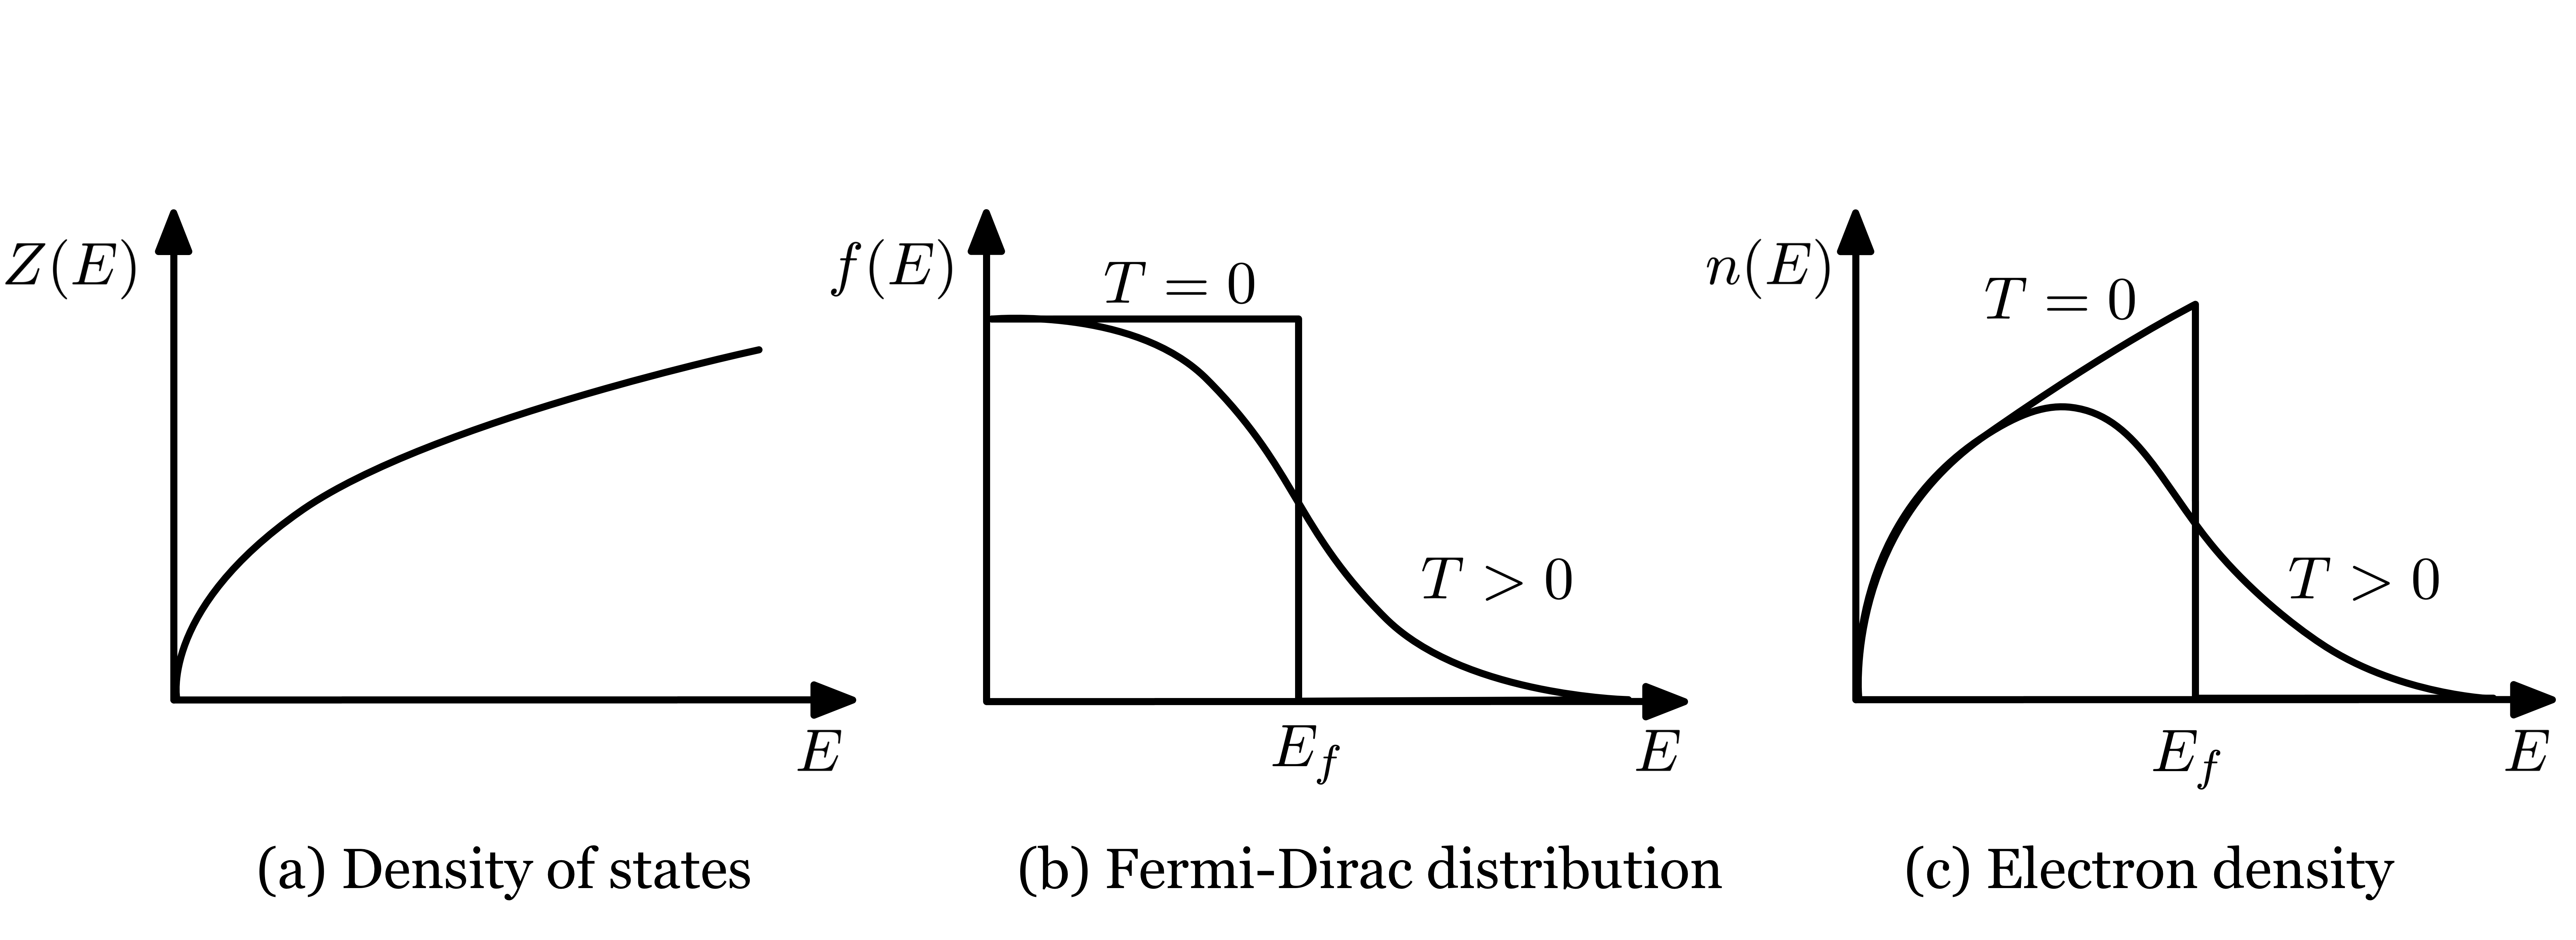
\includegraphics[width=0.9\linewidth]{files/density-fermidirac}
		\caption{Density of states a), Fermi-Dirac distribution b) and electron density c)}
		% \label{ }
		\end{figure}

		It is then fundamental to take into consideration, for semiconductors, the effect of band of available energy level and especially the band gap separating the conduction and valence band as follows: 
		\begin{equation}
			Z_n(E)dE = 4 \pi {\left(\frac{2m_n^*}{h^2}\right)}^{{3/2}} \sqrt{E-E_{C}}\ \Theta(E-E_C)dE
		\end{equation}
		\begin{equation}
			Z_p(E)dE = 4 \pi {\left(\frac{2m_p^*}{h^2}\right)}^{{3/2}} \sqrt{E_V-E}\ \Theta(E_V-E)dE
		\end{equation}

		The Heaviside function $\Theta$ accounts from the sudden transition at the band's edges to the gap. One can thus multiply the respective density of states for positive and negative charge carriers to the energy states distributions discussed in \eqref{eq:FermiDirac} to obtain the charge carrier concentration. 

		\begin{figure}[h]
			\centering
			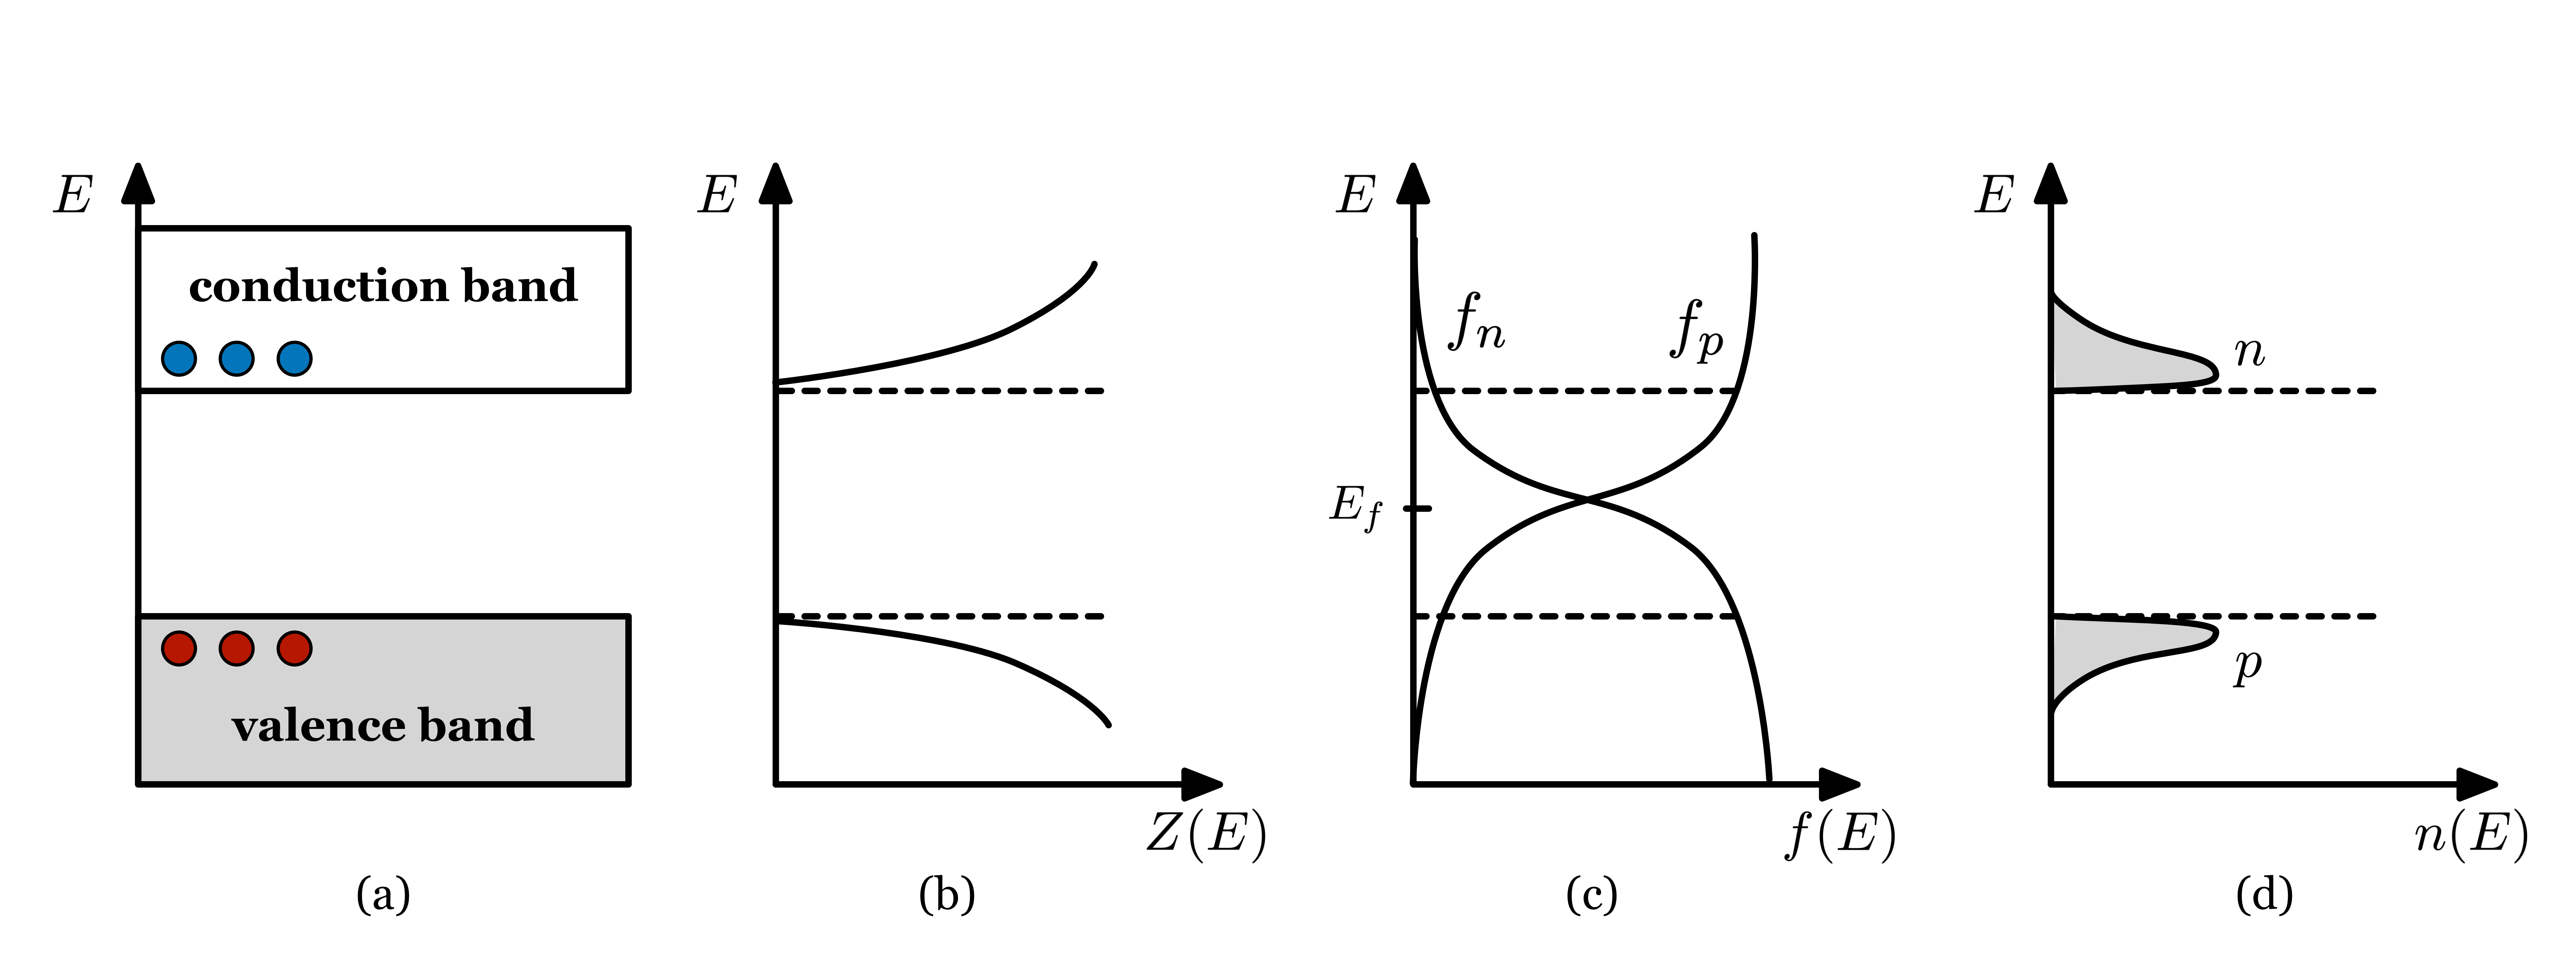
\includegraphics[width=0.95\linewidth]{files/band_diagram}
			\caption{Band diagram (a), Density of states (b), Occupation probabilities (c) and charge carrier densities (d)}
			% \label{ }
		\end{figure}

		For intrinsic semiconductors, a good approximation is to consider the Fermi energy level to be exactly in the middle of the band gap, this leads to having $(E-E_F) \gg kT$ and so  the expression for the occupation probabilities can be simplified as:
		\begin{equation}
			f_n(E) = \frac{1}{\exp(\frac{E-E_f}{kT}) + 1} \approx \exp(- \frac{E-E_f}{kT})
		\end{equation}

		It is then interesting to calculate the number densities $n$ and $p$ respectively for negative and positive charge carriers, integrating respectively over the conduction and valence band energies and using that by definition $f_n(E) + f_p(E) = 1$. This leads to: 
		\begin{equation}
			n = 2{\left( \frac{m_n^* kT}{2 \pi \hbar^2} \right)}^{3/2} \exp(-\frac{E_C - E_f}{kT}) \equiv N_C \exp(-\frac{E_C - E_f}{kT})
			\label{eq:ndensities_n}
		\end{equation}

		\begin{equation}
			p = 2{\left( \frac{m_p^* kT}{2 \pi \hbar^2} \right)}^{3/2} \exp(-\frac{E_f - E_V}{kT}) \equiv N_V \exp(-\frac{E_f - E_V}{kT})
			\label{eq:ndensities_p}
		\end{equation}

		For the sake of understanding, we can estimate the values of the effective densities of states, averaging over the effective masses of both charge carriers in Silicon and at room temperature (\SI{300}{\kelvin}) such that\ \cite{leroy2012silicon}: 
		\begin{equation}
			\begin{split}
				& N_C = 2 {\left( \frac{m_n^* kT}{2 \pi \hbar^2} \right)}^{3/2} \approx 3.05 \times 10^{19} \text{ cm$^{-3}$} \\
				& N_V = 2 {\left( \frac{m_p^* kT}{2 \pi \hbar^2} \right)}^{3/2} \approx 2.55 \times 10^{19} \text{ cm$^{-3}$}
			\end{split}
			\label{eq:effdensities}
		\end{equation}

		In thermal equilibrium, generation and recombination of electrons and holes respectively in the conduction and valence band are balanced which means: 
		\begin{equation}
			n = p = n_i \hspace{5mm} \Rightarrow \hspace{5mm} n \cdot p = n_i^2 = const
			\label{eq:massaction}
		\end{equation}

		In the case of unbalance between the number of positive and negative charge carriers (doping for instance could produce such an effect), we can use the expressions found in \eqref{eq:ndensities_n} and \eqref{eq:ndensities_p} to find: 
		\begin{equation}
			\begin{split}
				n_i^2 = np 	& = N_C N_V \exp(-\frac{E_C-E_V}{kT})\\
										& = N_C N_V \exp(-\frac{E_G}{kT})
			\end{split}
		\end{equation}
		The intrinsic carrier concentration depends on the difference of the energy levels of the conduction and valence band, the band gap energy, and has a dependence on the temperature such that: 
		\begin{equation}
			n_i \propto T^{3/2} \exp(\frac{-E_G}{2kT})
		\end{equation}
		Using the previously computed values for the effective densities of states in the conduction and valence band in \ref{eq:effdensities}, we find that at room temperature: 
		\begin{equation}
			n_i \approx 1.01 \times 10^{10} \text{ cm$^{-3}$}
		\end{equation}

		It is finally possible to give an expression to the Fermi level as a function of the energy levels of the conduction and valence bands and the effective masses fo electrons and holes, using that the concentration of both is equal: 
		\begin{equation}
			E_f = \frac{E_C + E_V}{2} + \frac{3kT}{4} \ln(\frac{m_p^*}{m_n^*})
		\end{equation}
		This results confirms that at $T =$ \SI{0}{\kelvin}, the Fermi level is exactly at the middle of the band gap and then slowly drifts away with increasing temperature due to the different in effective masses for electrons and holes. 
		To conclude the discussion on the electrical properties of intrinsic semiconductors, it is interesting to use the mobility of electrons and holes (respectively $\mu_e = $ \SI{1450}{\frac{\centi\meter\squared}{\volt\second}} and $\mu_h = $ \SI{500}{\frac{\centi\meter\squared}{\volt\second}}) to estimate the conductivity of intrinsic Silicon at room temperature: 
		\begin{equation}
			\sigma_i = n_i e {\left( \mu_e + \mu_h \right)} \approx 2.8 \times 10^{-4} \text{ ($\Omega$m)$^{-1}$}
		\end{equation}

		\subsubsection{Doping: extrinsic semiconductor}

		Extrinsic semiconductor are characterized by the addition of so-called impurities in the crystal's structure, the idea behind this doping of intrinsic semiconductors is to modify its conduction properties. Silicon being a tetravalent atom, it is possible to create an excess of electrons by replacing Silicon atoms by pentavalent atoms like Phosphorus (P) or Arsenic (As), these atoms are called donors.  Vice versa, it is possible to create an excess of holes by replacing Silicon atoms with trivalent atoms like Boron (B) or Gallium (Ga), these atoms are called acceptors.
		
		The mass-action law described in \eqref{eq:massaction} holds for doped semiconductors as the doping both increases the density of one type charge carrier and reduces the density of the other. Accounting for the fact that the net charge density of charge carriers for any volume element of semiconductor is zero, we obtain for the charge carrier densities as a function of the number of donor and acceptor atoms: 
		\begin{equation}
			\rho = e(n - p + N_A - N_D) = 0 \hspace{5mm} \Rightarrow \hspace{5mm} n-p = N_D - N_A
		\end{equation}
		
		Combining this relation to the mass-action law given in \eqref{eq:massaction}, one can derive the majority carrier densities and minority carrier densities in the cases in which electron (n-type semiconductor) or holes (p-type semiconductor) are dominating, respectively: 
		\begin{equation}
			n_n = \frac{1}{2} {\left( N_D - N_A + \sqrt{4 n_i^2 + (N_D - N_A)^2} \right)} \approx |N_D - N_A| \approx N_D
		\end{equation}
		\begin{equation}
			p_p = \frac{1}{2} {\left( N_A - N_D + \sqrt{4 n_i^2 + (N_D - N_A)^2} \right)} \approx |N_A - N_D| \approx N_A
		\end{equation}

		Equivalently, we can derive the minority carrier densities for holes and electrons respectively: 
		\begin{equation}
			p_n \approx \frac{n_i^2}{N_D - N_A} \approx \frac{n_i^2}{N_D} \hspace{5mm} ; \hspace{5mm} n_p \approx \frac{n_i^2}{N_A - N_D} \approx \frac{n_i^2}{N_A}
 		\end{equation}

		In n-type semiconductors, the addition of donor atoms for example will add some energy levels available slightly below the conduction band energy level so that new states will need to be accounted for in the density of states distribution. The Fermi level will then be raised from its intrinsic value $E_f$ to $E_F$ so that the population densities will change in favour of the electrons in the conduction band such that: 
		\begin{equation}
			n \approx N_D = N_C \exp(-\frac{E_C - E_f}{kT})\exp(-\frac{E_f - E_F}{kT}) = n_i \exp(-\frac{E_f - E_F}{kT})
		\end{equation}

		Equivalently, for p-type semiconductors: 
		\begin{equation}
			p \approx N_A = n_i \exp(\frac{E_f- E_F}{kT})
		\end{equation}
		The variation between the Fermi levels in the intrinsic and extrinsic cases is directly linked to the amount of donor or acceptors atoms. 
		Non desired impurities can also be present inside the crystalline structure as well as it is not straight forward to obtain a pure Silicon sample. Similarly, some different energy levels can be added and depending on their location in the band gap, they could act either as donors or acceptors.
		\clearpage
		\subsection{Junction and external voltage}\label{subsec:2.1.2}

		\begin{figure*}[h]
		\begin{minipage}{0.53\linewidth}
			A pn junction is created when bringing together p-type semiconductor and n-type semiconductor in contact. For the p-type side, the Fermi level is closer to the valence whereas for the n-type side, the Fermi level is closer to the conduction band. At the interface, the strong gradient in charge carrier concentration give rise to a diffusion current $I_{diff}$ such that electrons from the n-type side diffuse in the p-type side and vice versa for holes. Due to recombination of both charge carrier types around the interface, a zone free of space charge is generated: the depletion zone. The ionised donor and acceptors atoms are still present in the lattice and an intrinsic electrical field will be generated, resulting in a drift current $I_{drift}$ in opposition to the diffusion current. 	
		\end{minipage}\hfill
		\begin{minipage}{0.45\linewidth}
			\centering
			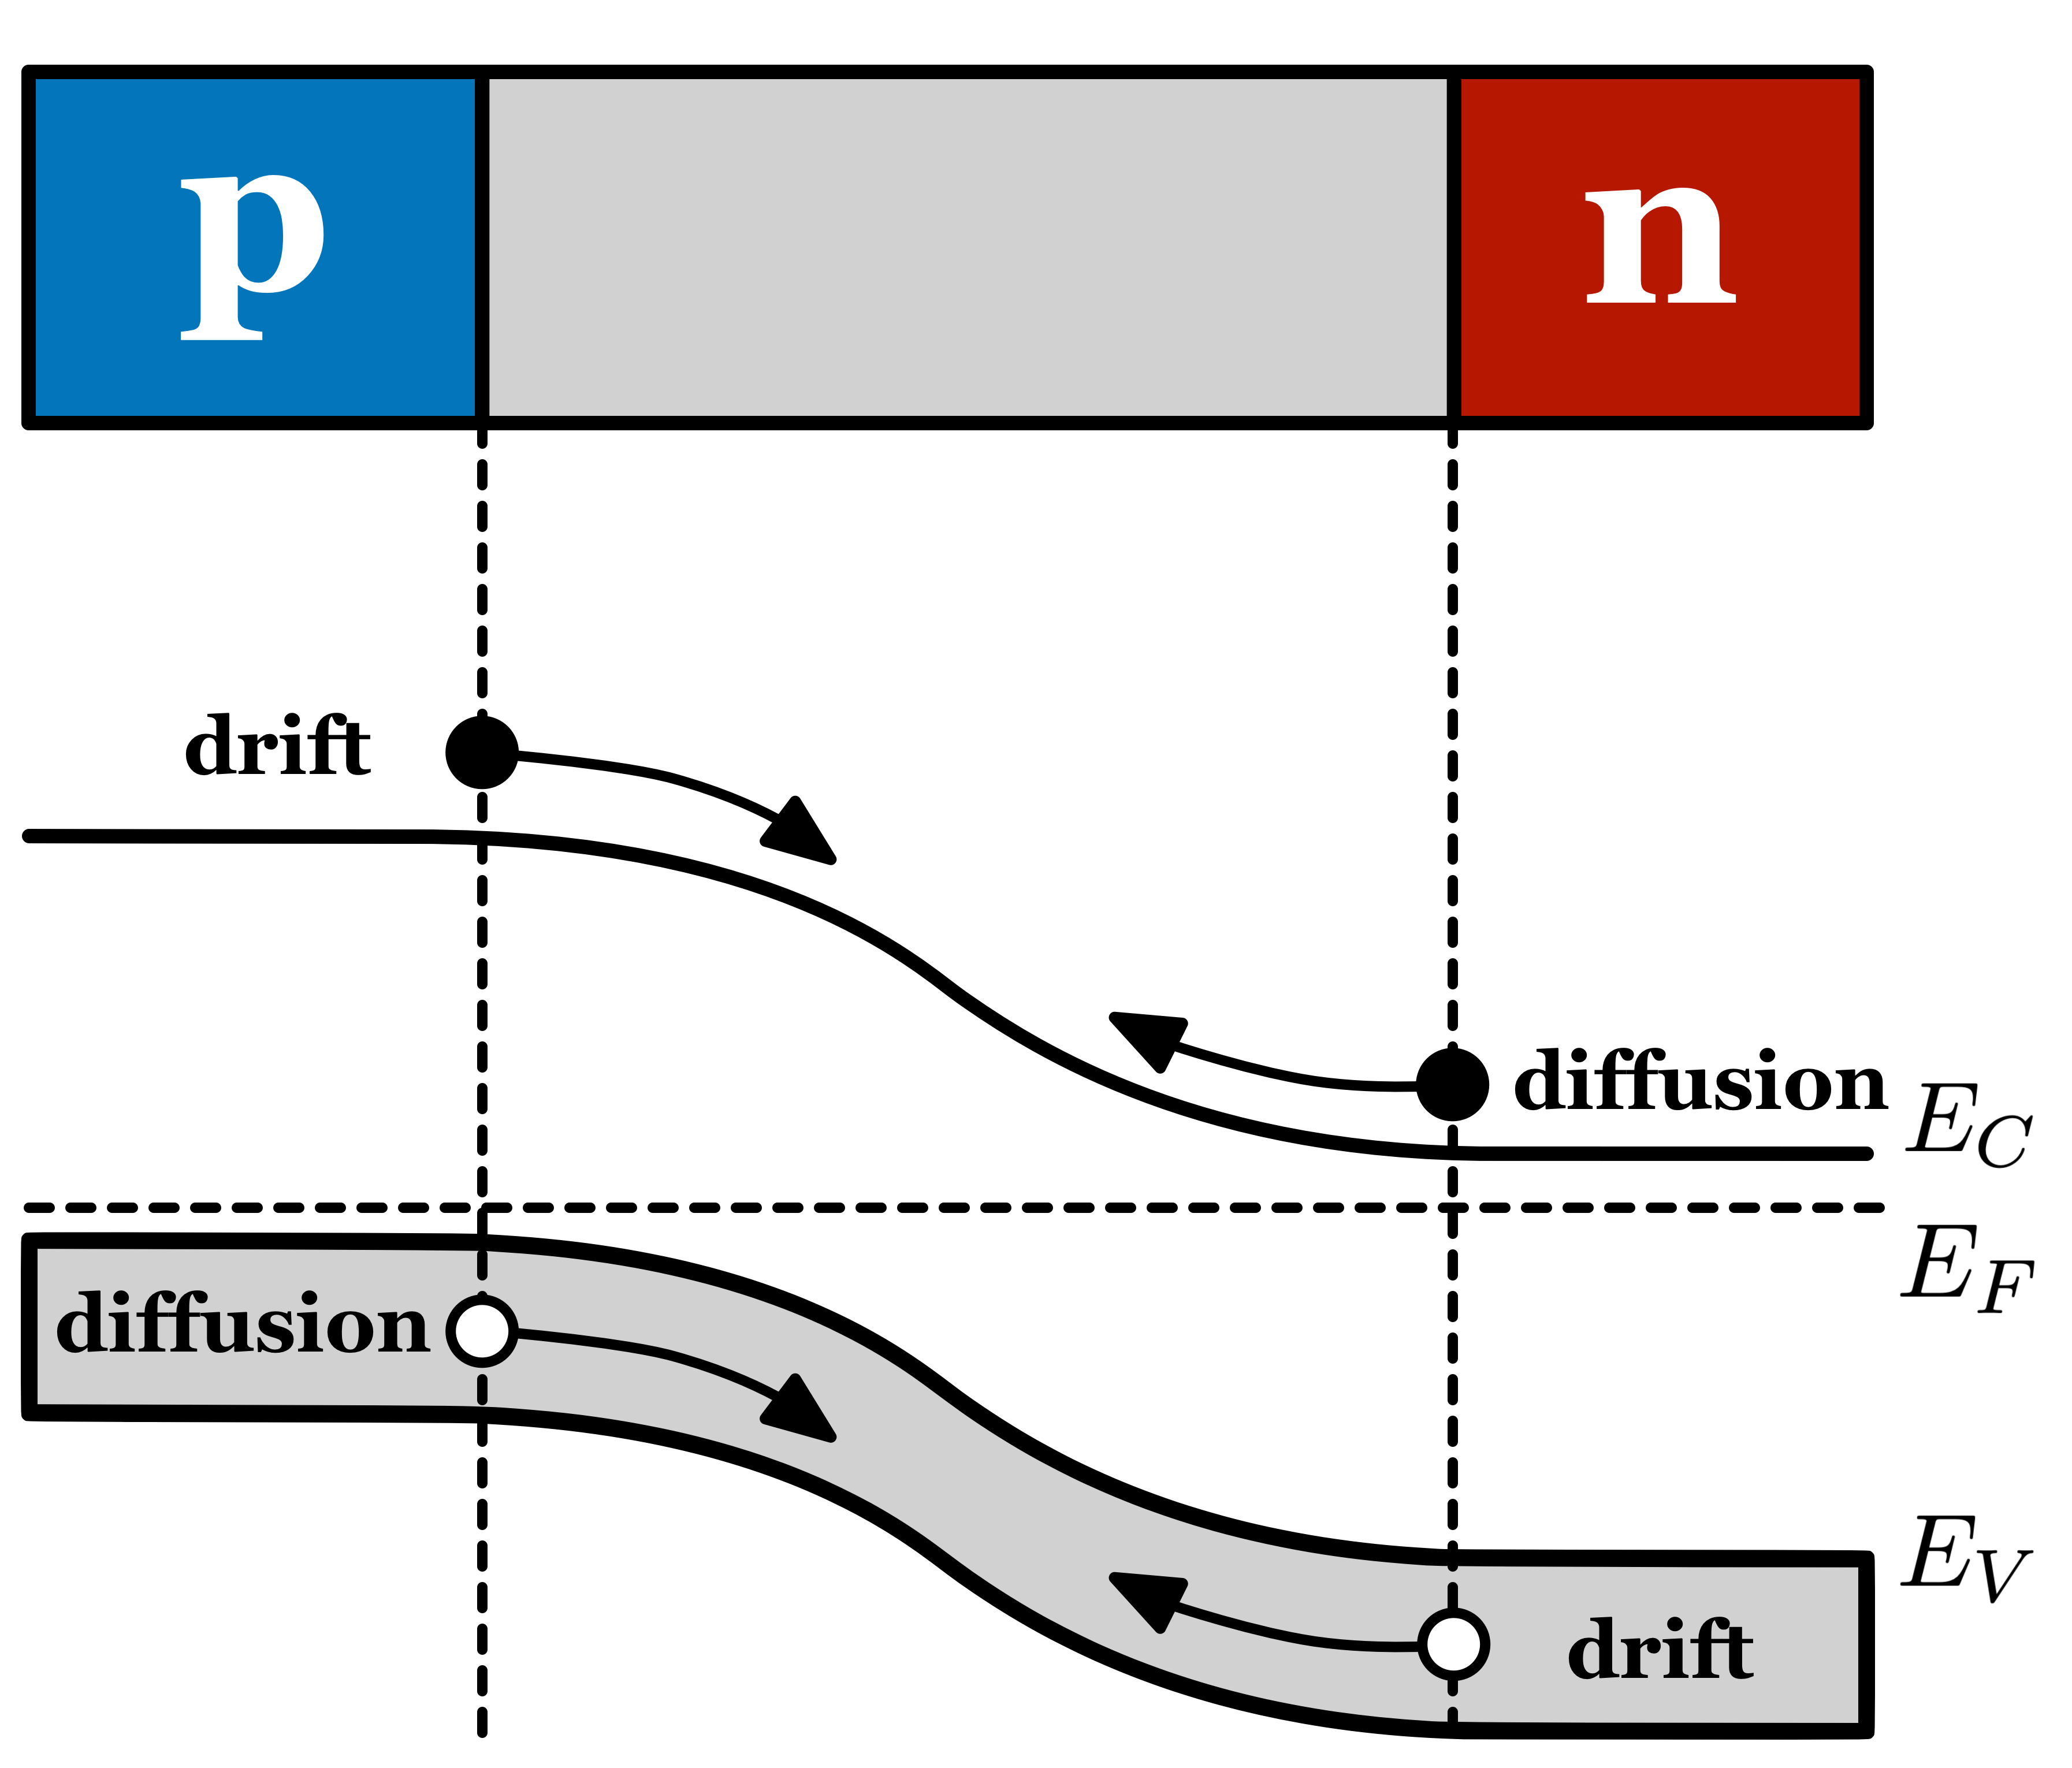
\includegraphics[width=1.0\linewidth]{files/band_structure}
			\caption{Band structure, potential and electric field of pn junction }
			\label{ }
		\end{minipage}
		\end{figure*}
		
		The resulting built-in electrical potential ($V_{bi}$) will produce a bending of the energy levels of the valence band and conduction band across the depletion region while the Fermi level will remain constant by its definition. 
		In equilibrium, the charge density can be written as: 
		\begin{equation}
			\rho(x) = 
			\begin{cases}
				-eN_A, & \text{for } -x_p < x < 0 \\
				+eN_D, & \text{for } 0 < x < x_n
			\end{cases}
		\end{equation}

		From the above equation and the neutrality condition $N_A x_p = N_D x_n$, one can derive the expression of the electric field $\mathcal{E}(x)$, imposing that the field has to be zero at the boundaries defined by $x_p$ and $x_n$ such that: 
		\begin{equation}
			\frac{d\mathcal{E}(x)}{dx} = \frac{\rho(x)}{\epsilon \epsilon_0} \hspace{4mm} \Rightarrow \hspace{4mm} \mathcal{E}(x) = 
			\begin{cases}
				\frac{-eN_A}{\epsilon \epsilon_0} (x + x_p) & \text{for } -x_p < x < 0 \\
				\frac{+eN_D}{\epsilon \epsilon_0} (x - x_n) & \text{for } 0 < x < x_n
			\end{cases}
			\label{eq:intrinsicEfield}
		\end{equation}

		By definition, the field maximum $\mathcal{E}_{max}$ is found at $x=0$. The built-in voltage can be derived through the integration of the intrinsic electric field obtained in \eqref{eq:intrinsicEfield} in the range defined by $x_p$ and $x_n$: 
		\begin{equation}
			\begin{split}
				V_{bi} = - \int_{-x_p}^{x_n} \mathcal{E}(x)dx &= \frac{e}{2 \epsilon \epsilon_0} (N_A x_p^2 + N_D x_n^2) \\
																											&= \frac{e}{2 \epsilon \epsilon_0} x_p^2 \frac{N_A}{N_D}(N_A + N_D)
			\end{split}
		\end{equation} 
		
		A useful definition of the built-in potential is through the difference in potential in the $n$ region $\phi_n$ and $p$ region $\phi_n$ around the depletion zone $V_{bi} = \phi_p - \phi_n$. The potential itself can be defined as the difference of extrinsic Fermi level $E_F$ and intrinsic Fermi level $E_f$ in both regions, such that:		 
		\begin{equation}
			\begin{split}
				V_{bi}  &= \phi_n - \phi_p = \frac{kT}{e}\ln(\frac{N_A}{n_i}) +\frac{kT}{e}\ln(\frac{N_D}{n_i})\\
								&=  \frac{kT}{e}\ln(\frac{N_A N_D}{n_i^2})
			\end{split}
			\label{eq:built-inpot}
		\end{equation} 

		To conclude this discussion it is interesting to compute the position of the boundaries of the depletion zone $x_n$ and $x_p$ as a function of the built-in potential and the donor and acceptor densities: 
		\begin{equation}
			x_p = \sqrt{\frac{2 \epsilon \epsilon_0}{e} V_{bi} \frac{N_D}{N_A(N_D + N_A)}} \hspace{5mm} \text{and} \hspace{5mm} x_n = \sqrt{\frac{2 \epsilon \epsilon_0}{e} V_{bi} \frac{N_A}{N_D(N_D + N_A)}}
		\end{equation}
		We observe that the depletion region is larger in the side of the junction where the doping is the lightest. Usually, the difference in doping concentrations is such that one can neglect for n-type (p-type) the density of donors (acceptors) and hence simplify the expression above. 

		\subsubsection{Effect of external voltage}
		
		Under equilibrium conditions, the width of the depletion zone is proportional to the amount of donor and acceptor atoms in the two sides of junctions but also to the built-in voltage generated from the movement of charge carrier within the junction. Although, if one was to apply an external difference in voltage $V_{ext}$ at the edges of the junction, the system would no longer be in equilibrium and charge carriers would start to move depending on the polarity of the voltage itself. We can hence consider the two following situations: 
		\begin{itemize}
			\item \textit{Forward-bias}: The applied external voltage $V_{ext}$ is negative on the n-side with respect to the p-side, more electrons will diffuse from the n-side to the p-side and vice versa for holes. The result is a reduction in the built-in potential and hence a reduction in the width of the depletion zone and a weaker bending of the energy bands. 
			\item \textit{Reverse-bias}: The applied external voltage $V_{ext}$ is positive on the n-side with respect to the p-side, more electrons will be removed from the n-side and vice versa for holes. The result is an increase in built-in potential and hence an increase in the width of the depletion zone and a stronger bending of the energy bands. 
		\end{itemize} 

		\begin{figure}[h]
		\centering
		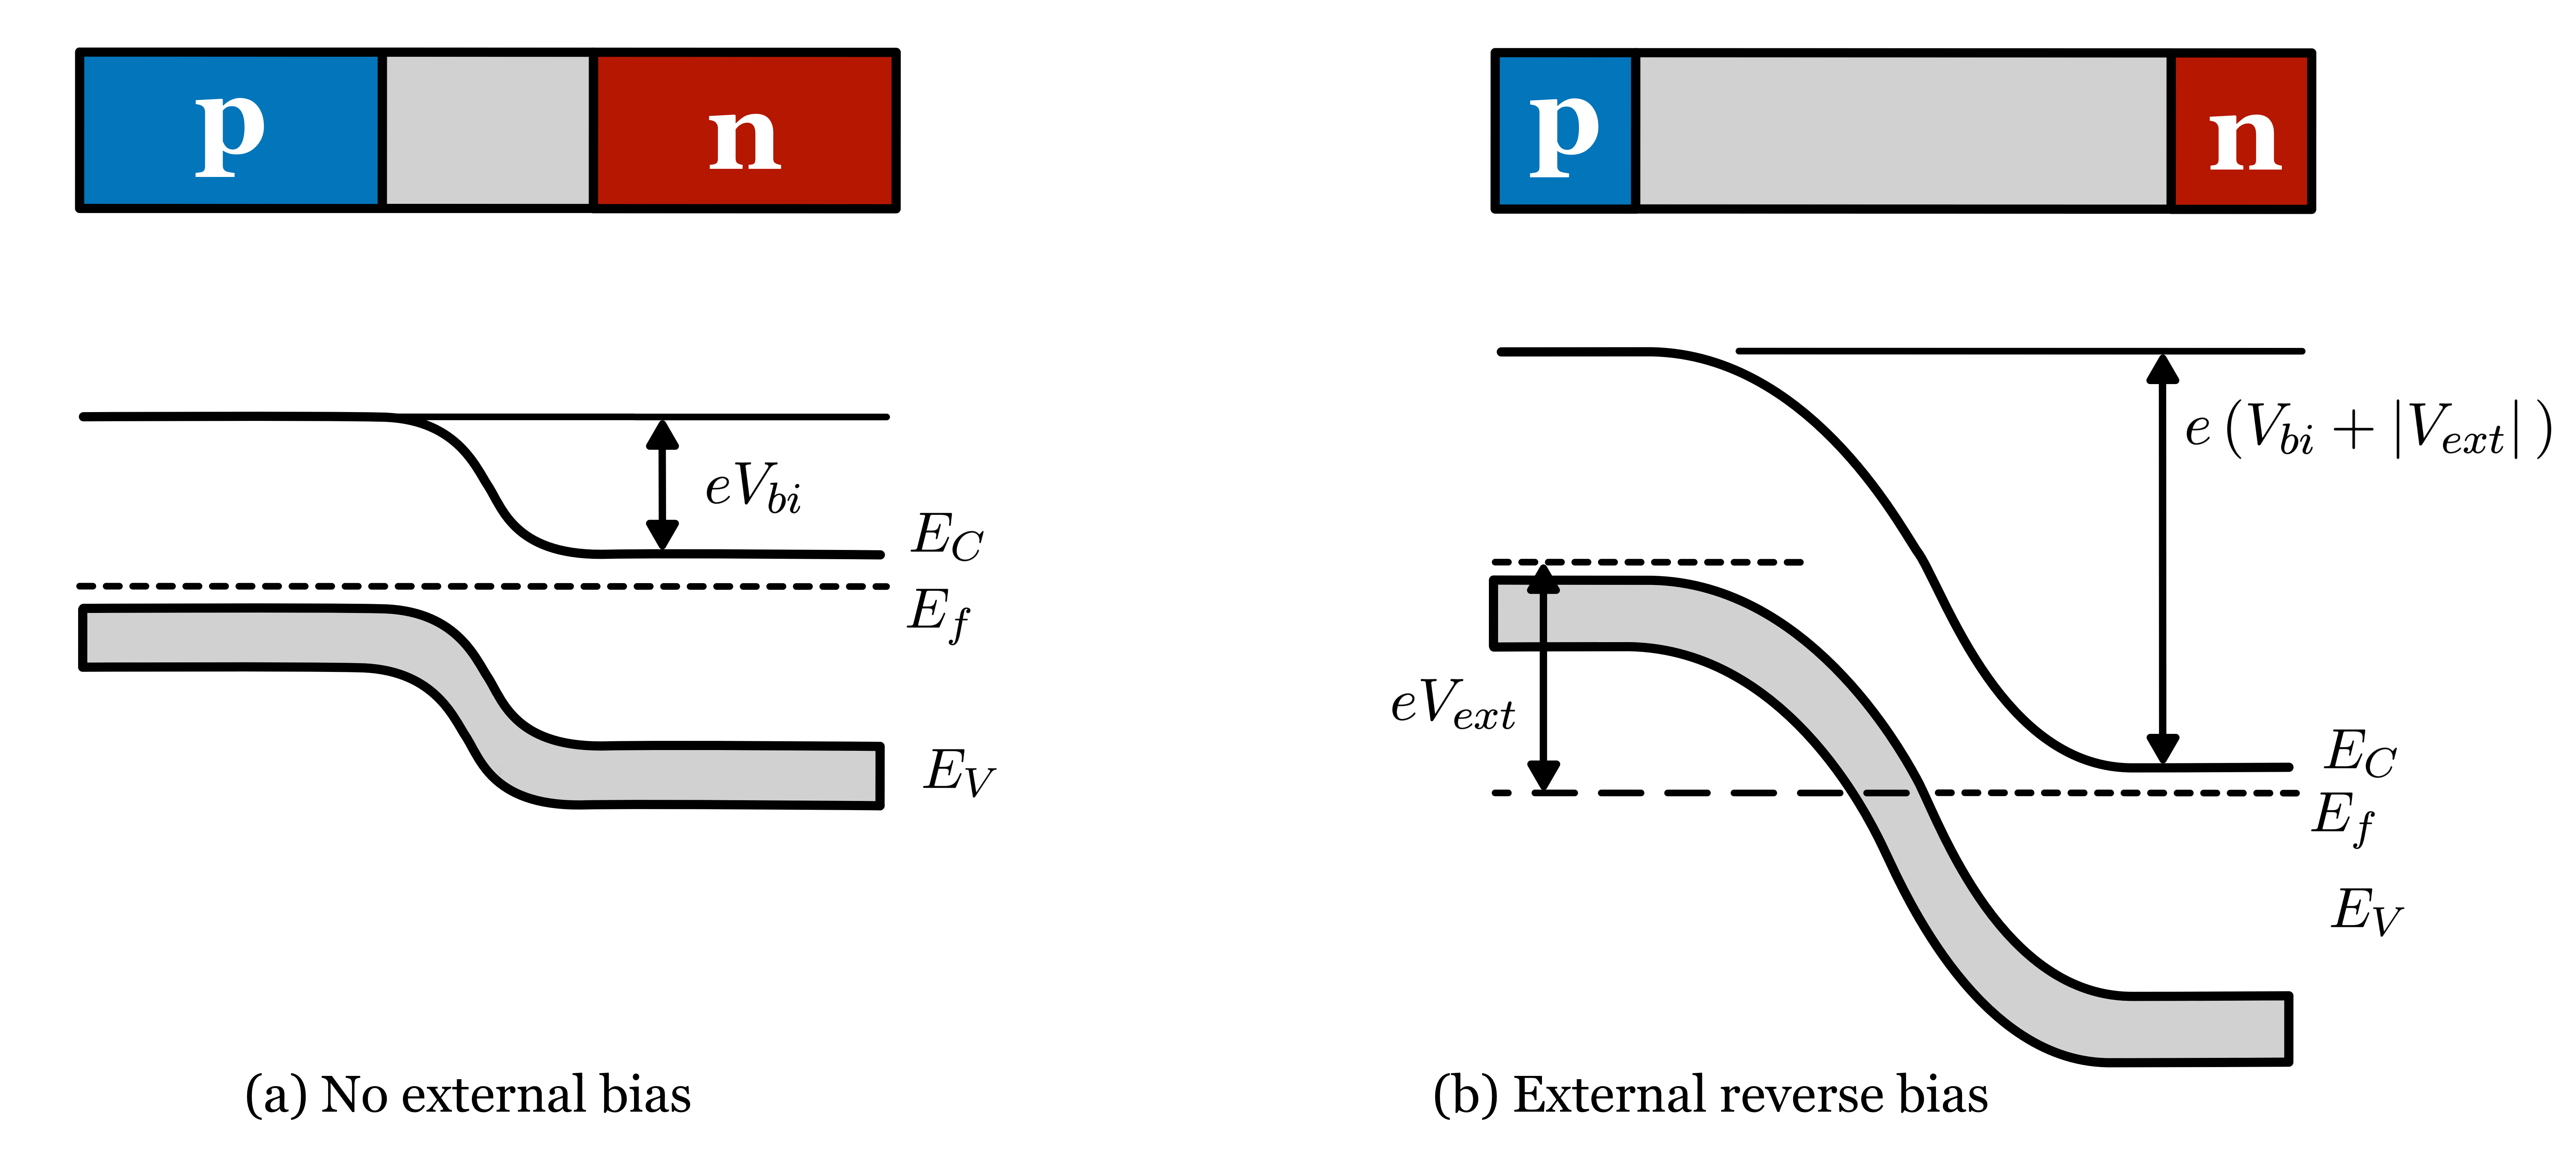
\includegraphics[width=1.0\linewidth]{files/pn_external_voltage}
		\caption{Effect of external voltage on a pn junction's band structure}
		\label{ }
		\end{figure}

	Outside the depletion region, equilibrium conditions hold and the concentration of majority carriers can be given by the donor and acceptor concentrations $N_A$ and $N_D$. 
	\clearpage
	Using the mass-action law, the expression for the built-in voltage from \eqref{eq:built-inpot} can then be adapted such that: 
	\begin{equation}
		V_{bi} = \frac{kT}{e} \ln(\frac{N_A N_D}{n_i^2}) \approx \frac{kT}{e} \ln(\frac{p_{p, eq} n_{n, eq}}{n_i^2}) = \frac{kT}{e} \ln(\frac{n_{n, eq}}{n_{p, eq}}) = \frac{kT}{e} \ln(\frac{p_{p, eq}}{p_{n, eq}})
	\end{equation}
	We have in the above equations defined the majority carrier concentrations in the n-side and p-side regions respectively as $n_{n, eq} \approx N_D$ and $p_{p, eq} \approx N_A$ and also the minority charge carriers, in the n-side and p-side regions, respectively as $n_{p, eq}$ and $p_{n, eq}$. One can first express the majority carrier densities in the region outside the space-charge region and then assume that these later are defined at the space charge boundaries by the difference $V_{bi} - V_{ext}$, such that: 
	\begin{equation}
		n_n(x = x_n) = n_p \exp(\frac{e(V_{bi} - V_{ext})}{kT}) \approx n_{n, eq}
	\end{equation}
	\begin{equation}
		p_p(x = -x_p) = p_n \exp(\frac{e(V_{bi} - V_{ext})}{kT}) \approx p_{p, eq}
	\end{equation}
	It is then possible to express this time the concentration of electrons at the boundary of the space-charge region on the p-side and the hole concentration at the opposite boundary on the n-side so that one obtains: 
	\begin{equation}
		n_p(x = -x_p) = n_{p, eq} \exp(\frac{e V_{ext}}{kT})
	\end{equation} 
	\begin{equation}
		p_n(x = x_n) = p_{n, eq} \exp(\frac{e V_{ext}}{kT})
	\end{equation}

	While reversed-bias is applied to the junction, the concentration of the majority charge carriers drop well below the minority charge carriers concentration in equilibrium and can be easily neglected in situation with high reversed-bias applied. Throughout the depletion region, the carrier concentration decreases from the majority carrier value $p_p (n_n)$ on one side, down to the minority carrier value $p_n (n_p)$ on the other side. The functional progression of the concentration into the depletion zone is determined by the concentration values at the end of the depletion region, that is, the transition to neutral regions. In summary, they are determined by the donor and acceptor concentrations and the external voltage applied to the junction\ \cite{detectors} 

	As it was discussed previously for the junction under no external voltage, it is possible to compute the depletion width of depletion zone and understand how it is affected. Respectively for the depletion zone boundary on the n-side or p-side, one obtains: 
	\begin{equation}
		d_{n} \approx x_n \approx \sqrt{\frac{2 \epsilon \epsilon_0}{e} \frac{1}{N_D}(V_{bi} - V_{ext})} \hspace{5mm} ; \hspace{5mm} d_{p} \approx x_p \approx \sqrt{\frac{2 \epsilon \epsilon_0}{e} \frac{1}{N_A}(V_{bi} - V_{ext})}
	\end{equation}
	A more convenient expression of the depletion width is through the use of the wafer resistivity which can be approximated as $\rho \simeq (e \mu_{e,h} N_{N_(D,A)})$, such that we obtain: 
	\begin{equation}
		d_n \approx 0.55 \sqrt{\frac{\rho}{\Omega cm} \frac{V_{ext}}{V}} \mu m \hspace{5mm} ; \hspace{5mm} d_{p} \approx 0.32 \sqrt{\frac{\rho}{\Omega cm} \frac{V_{ext}}{V}}  \mu m
		\label{eq:depletion_width}
	\end{equation}

	The difference between the p-side and n-side is due to the difference in mobility of electrons and holes, in order to deplete for example a silicon detector with \SI{300}{\micro\meter} width and a substrate resistivity of $\rho = $ \SI{2}{\kilo\ohm\centi\meter}, an external reverse bias voltage of \SI{160}{\volt} would need to be applied. 
\clearpage
	\subsubsection{Junction capacitance and full depletion}
		
	It is possible to treat the junction with a zone free of charge carriers just like a plate capacitor filled with a dielectric. The capacitance of the junction can then be given as a function of the area $A$ of the section of the junction and $d$ the width of the depletion zone by the following equation: 
		\begin{equation}
			\frac{C}{A} = \frac{\epsilon \epsilon_0}{d}
		\end{equation}

	We have seen previously that the depletion zone width depends on the applied external voltage \eqref{eq:depletion_width}. If one was to measure the capacitance as a function of the external bias supplied to the junction, it would be possible to find the tension for which the junction is fully depleted, since the capacitance would then become constant, we call this tension the full depletion voltage. 
	\begin{figure*}[h]
		\centering
			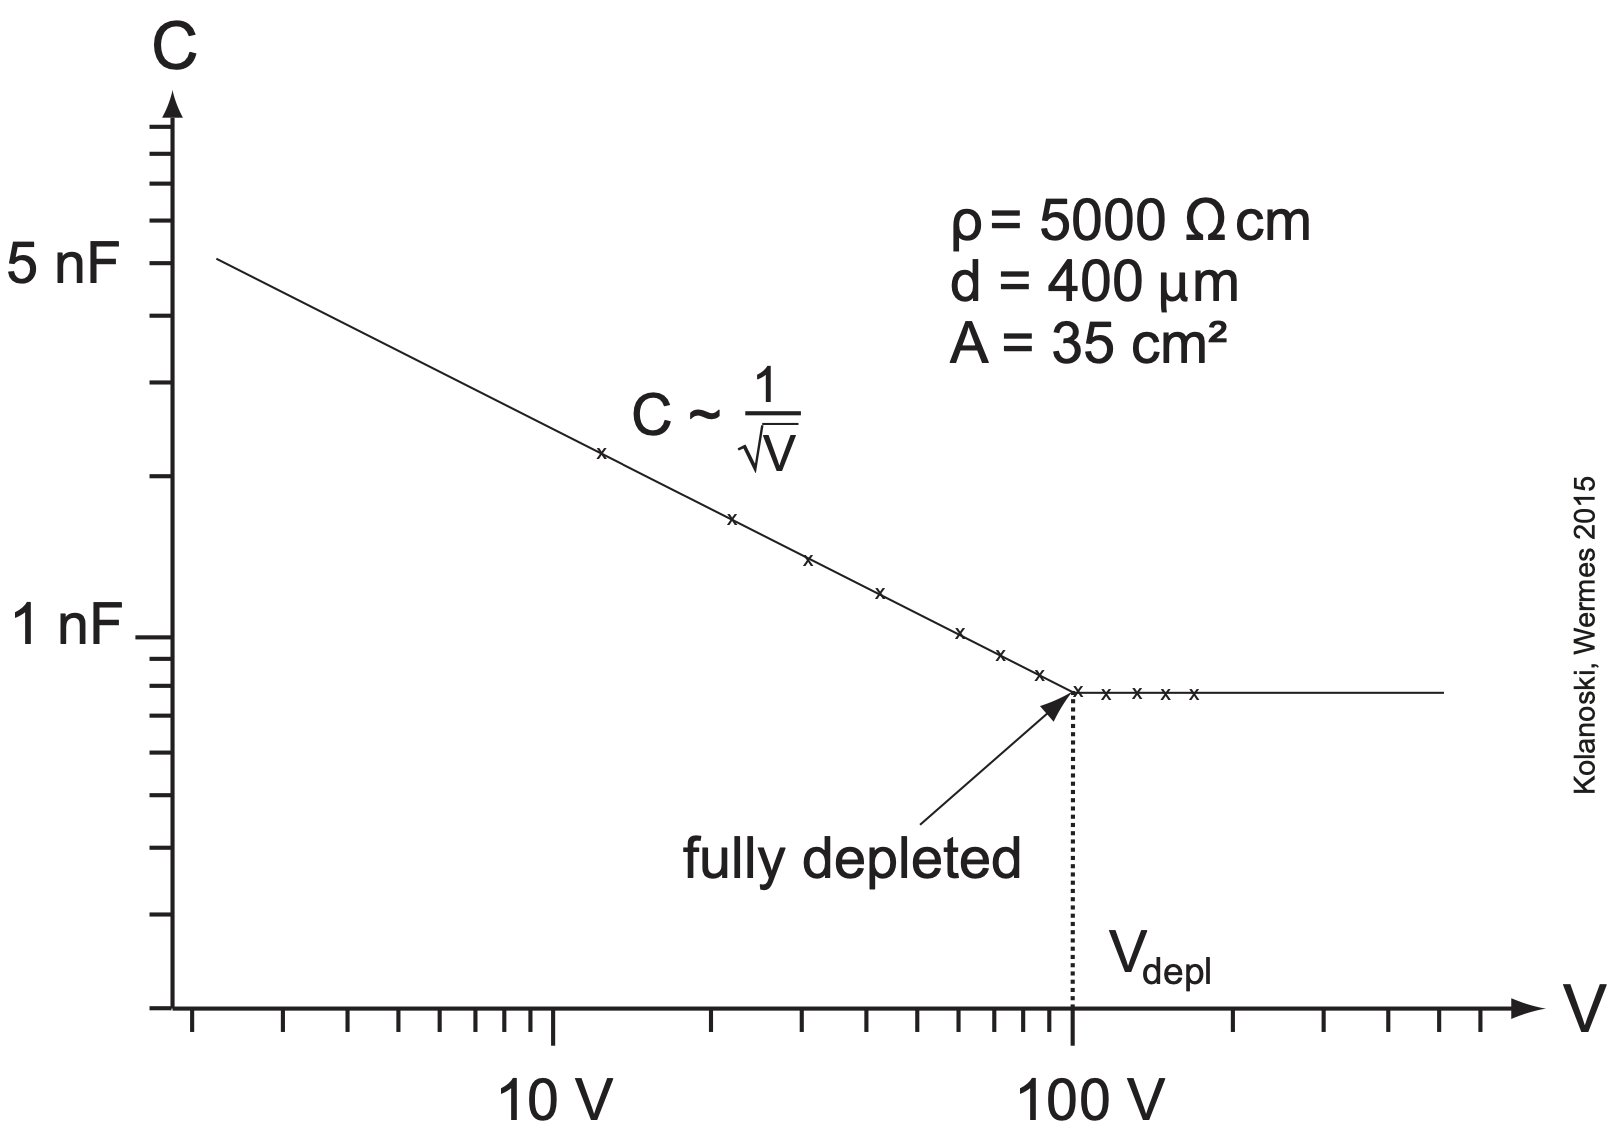
\includegraphics[width=0.6\linewidth]{files/CV_silicon}
			\caption{C-V curve of a silicon device in reverse bias}
			\label{ }
	\end{figure*}

	
	\clearpage
	\section{Signal formation and charge carrier transport}\label{sec:2.2}
		
	We previously discussed that it is possible to create with a pn junction, a region free of charge carriers, the so-called space charge region and that the width of this later can be adjusted by applying an external tension to the junction. While applying a reversed bias to the junction, one will increase the width of the space charge region. If a charged particle or a photon was to cross this region, some of the deposited energy would contribute to the creation of electron-hole ($e^- / h^+$) pairs. The energy required to generate a pair is temperature dependent but a commonly used value at room temperature is $\Delta E = \SI{3.6}{\electronvolt}$. Electrons and holes would then drift under the influence of the electric field inside the depletion region and could be collected on a readout electrode to observe the signal generated by the passage of this particle. 

	This is a very rough description of how semiconductors can be used for particle detection, in what follows we will give a more formal description of the drift of electrons and holes once they are generated, how the signal is induced at the electrodes and how the signal is formed.   

		\subsection{Drift of electrons and holes}\label{subsec:2.2.1}
		
		Motion of charges in semiconductors can be described by the Boltzmann transport equation as it takes into account both diffusion and drift mechanisms. Although, one also need to consider the lattice nature of semiconductors, implying that electrons and holes can be treated as if they were moving freely by using their effective mass as defined in \eqref{eq:effective_mass}. In semiconductors, the drift motion is a result of the acceleration of electrons and holes by the and electric field, moderated by friction and collision processes with the lattice phonon and impurities. The diffusion motion comes from the movement of charge carriers from a zone with lower concentration as it was discussed in \subsecref{subsec:2.1.2}

		For semiconductor particle detectors, the main process is the drift of electrons and holes induced by the external electric field induced by operating the devise in reversed-bias configuration. As said before, the motion can be described through the Boltzmann transport equation, but an often used description comes from using the Drude model \cite{Drude} which states that: 
		\begin{equation}
			m^* {\left( \dot{\vec{v}}_D + \frac{\vec{v}_D}{\tau}\right)} = q \vec{E}
		\end{equation} 
		We have here introduced as $\vec{v}_D$ the drift velocity and the various scattering effects are described by a relaxation parameter $\tau$, defined as the time separating two momentum changes between one scattering incidence and another. 
		
		\begin{figure*}[h]
			\centering
			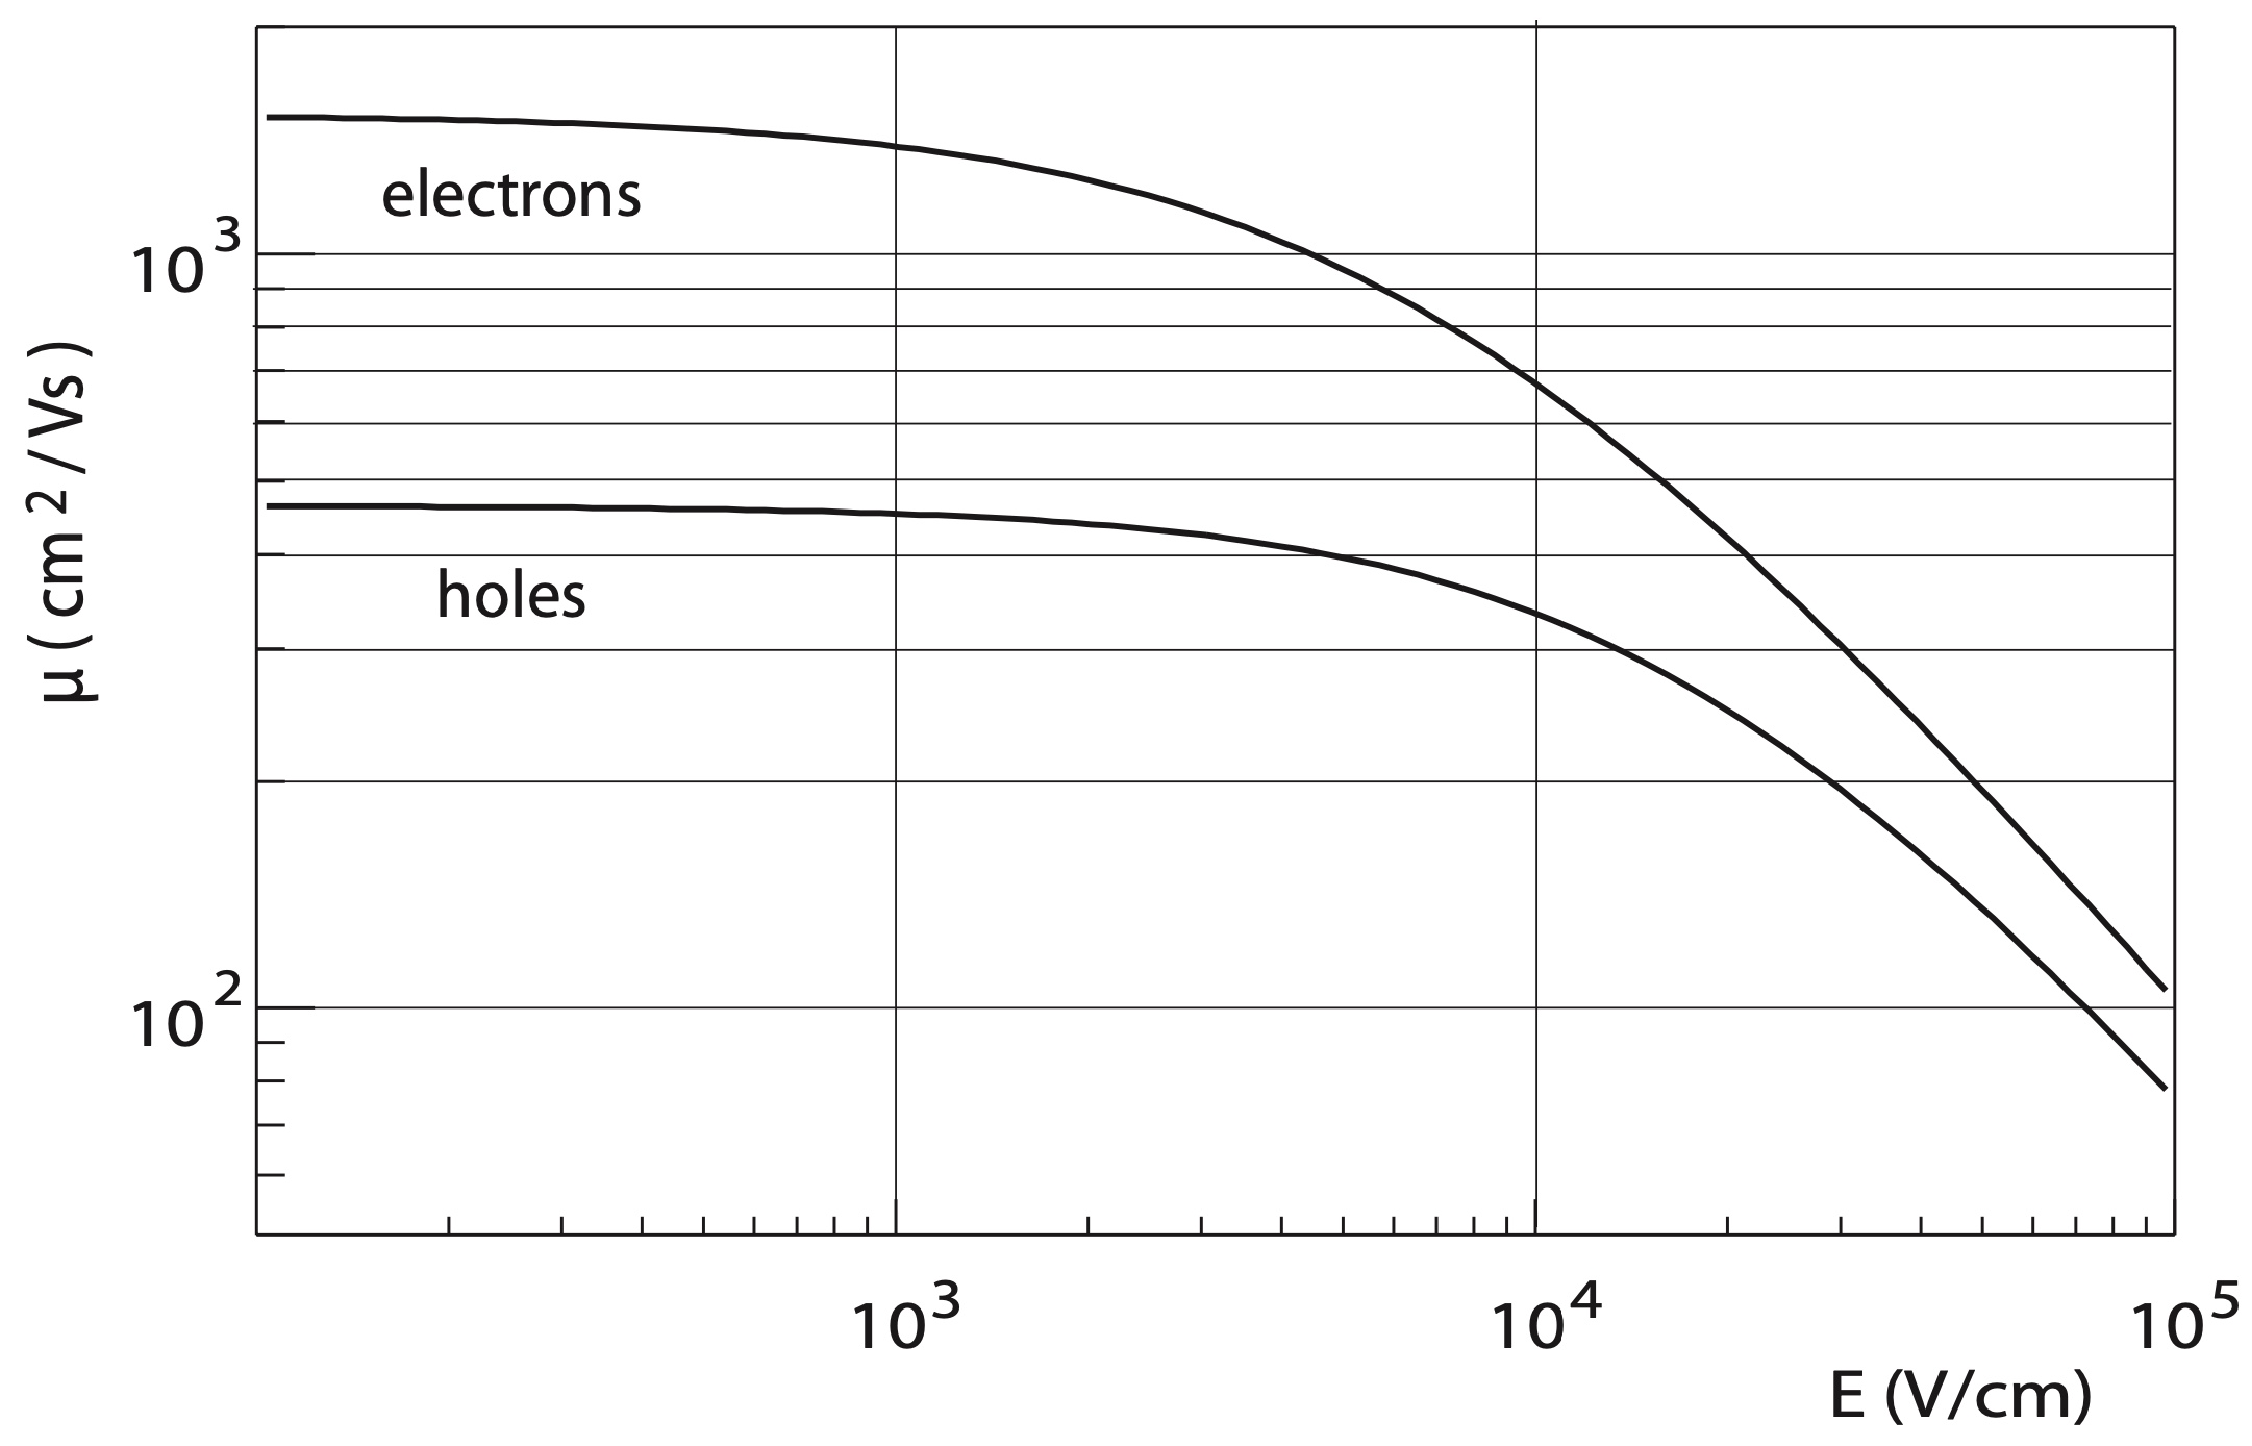
\includegraphics[width=0.58\linewidth]{files/electron-hole_mobility}
			\caption{ Mobilities of electron and holes in Silicon}
			\label{ }
		\end{figure*}

		If one assumes the stationary case of constant drift velocity, one can introduce the electron and hole mobility so that: 
		\begin{equation}
			\vec{v}_D = \frac{q \tau}{m^*} \vec{E} = \mu \vec{E} \hspace{5mm} \text{and} \hspace{5mm} \mu_{e,h} = \frac{q\tau}{m^*_{e,h}}
		\end{equation}
		
	
	

		The mobility of charge carriers is a temperature dependent quantity because of the temperature dependence of the different collisions processes defining the collision time $\tau$. As mentioned before, we can distinguish the collisions involving acoustic phonons (coherent lattice oscillations) for which the mobility decreases for increasing temperature, and the collisions involving impurities in the lattice, for which the mobility increases (weakly decreases) for collisions with charged (neutral) impurities.  

		The mobility of charge carriers also depends on the electric field present within the depletion region, at low electric fields ($E \ll \SI{10}{\kilo \volt \per \centi\meter}$), the drift velocity is proportional to the electric field whereas at high electric fields, the mobility is field dependent. At low electric field, thermal equilibrium can be assumed and the emission and absorption of phonons by charge carriers lead to almost no deviation from the proportionality to the electric field. With increasing electric field, a stationary equilibrium is reached between the energy spent for the acceleration of the charge carriers and the energy transferred to the lattice phonon scattering, the drift velocity eventually becomes constant (for Silicon at least). A sufficiently simple empirical ansatz gives a good description of the drift's velocity dependence on the electric field\ \cite{drift_velocity_vs_E}: 
		\begin{equation}
			\vec{v}_D = \mu(E) \vec{E} = \frac{\mu_0}{{\left(1 + {\left( \frac{\mu_0 E}{v_{sat}} \right)^\beta}\right)^{1/\beta}}} \vec{E}
			\label{eq:drift_velocity}
		\end{equation}
		We have here introduced $\mu_0$ the mobility at low electric field values, $v_{sat}$ the saturated drift velocities reached for high electric fields and an empirical constant $\beta$ which is usually taken to be 2 for electrons and 1 for holes in Silicon \cite{beta_drift_velocity}.  
		
		\begin{figure*}[h]
			\centering
			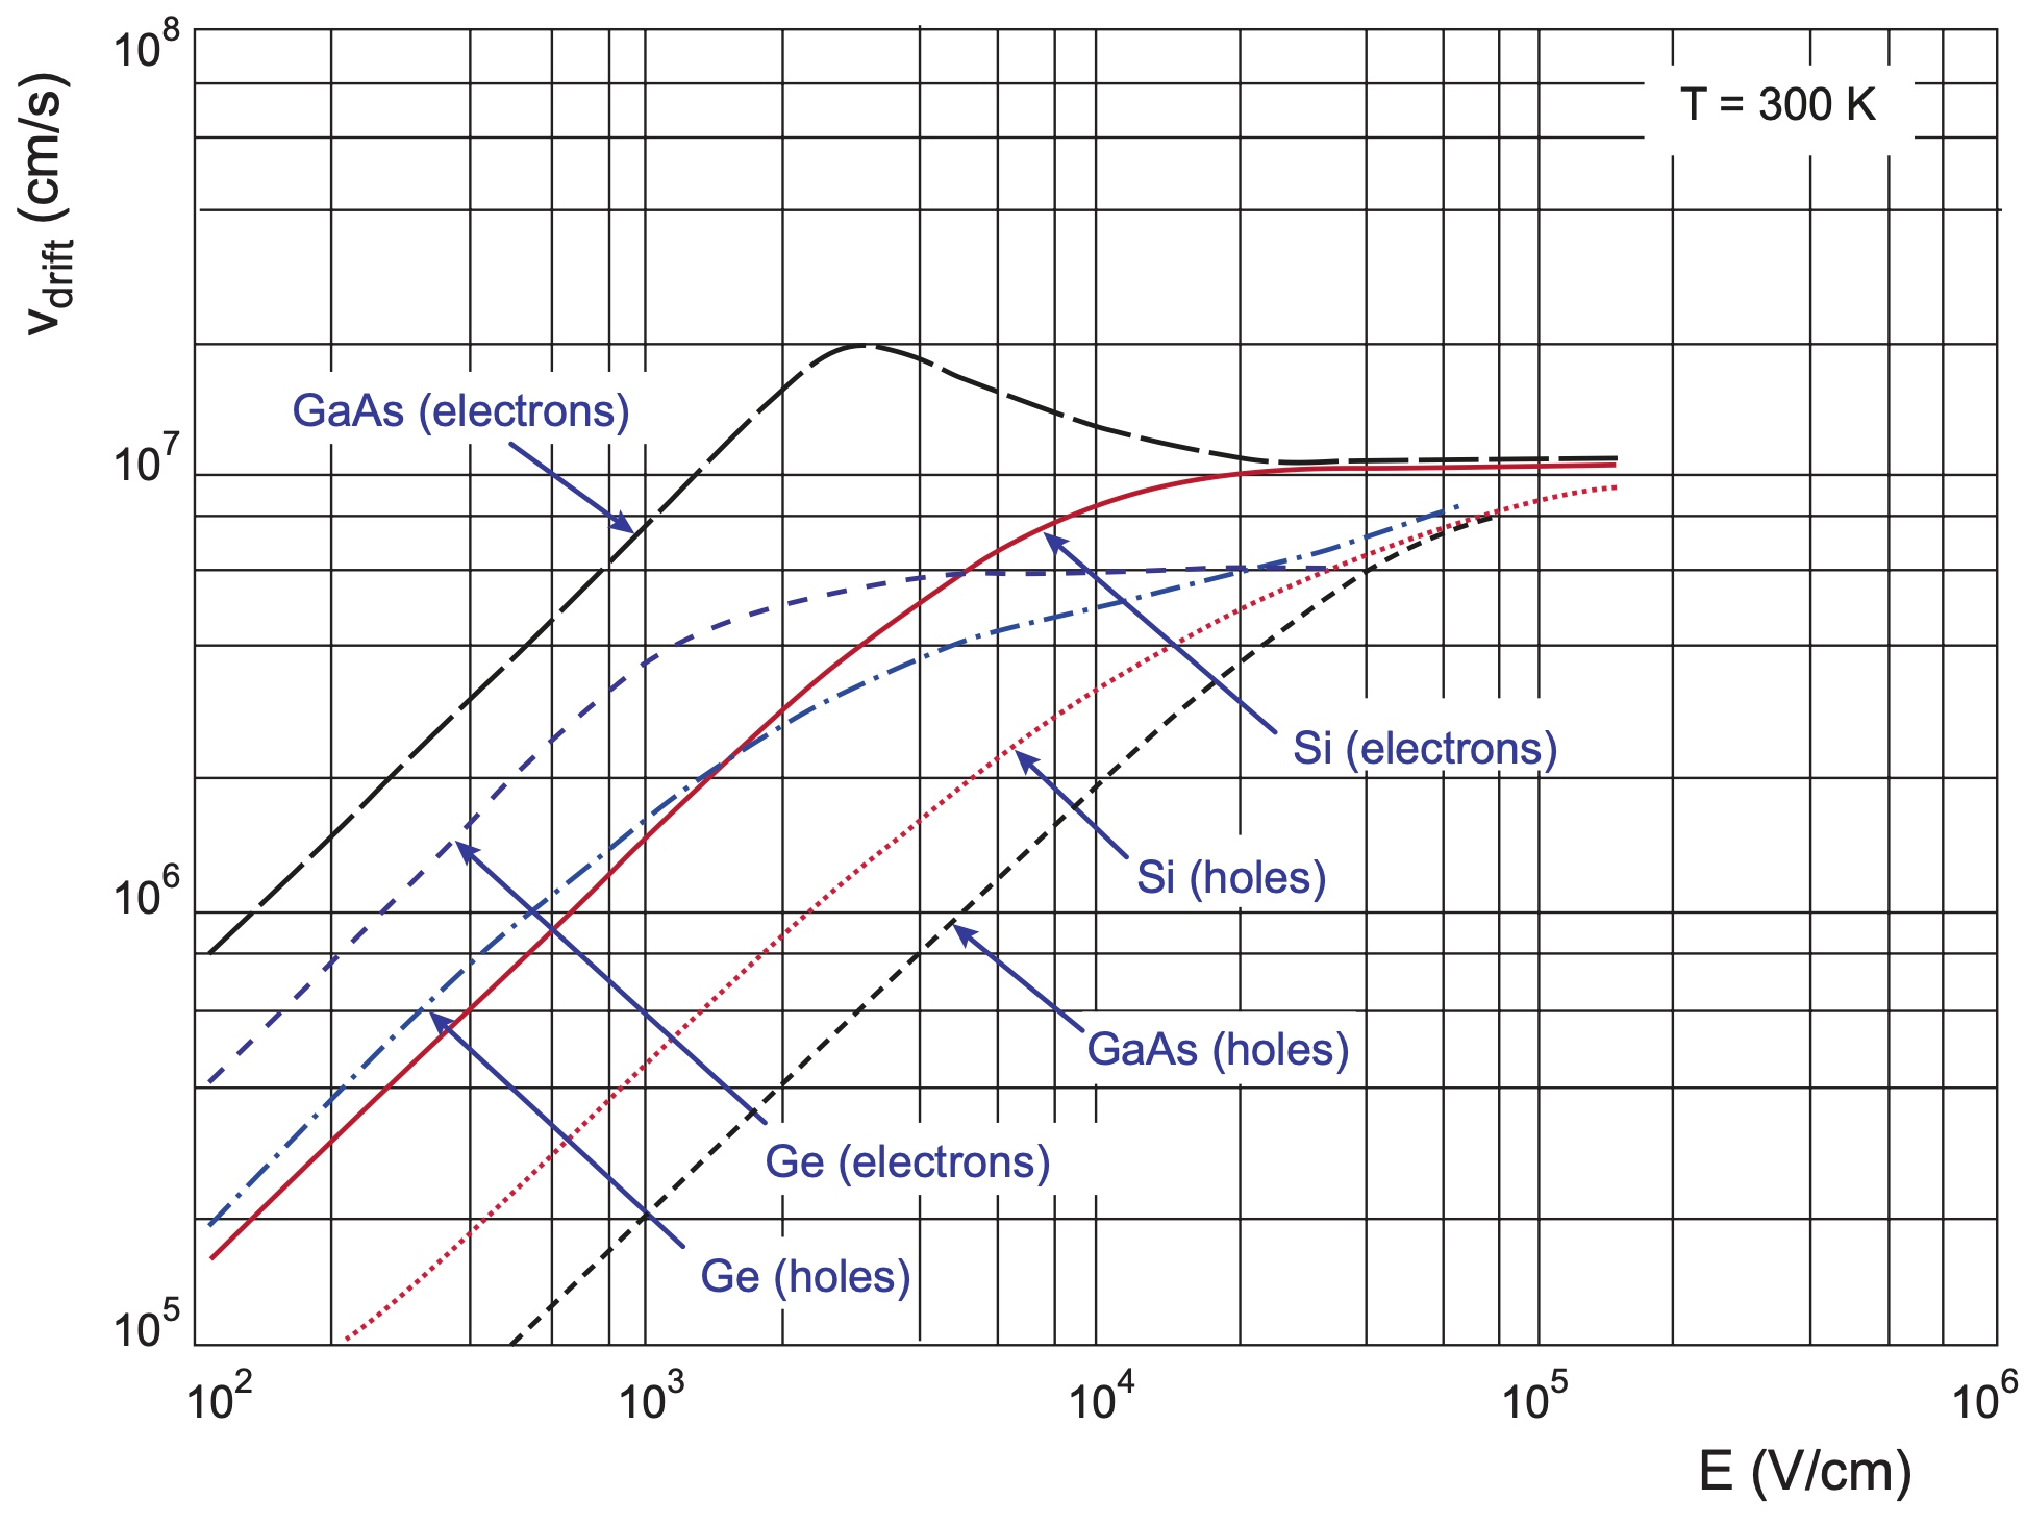
\includegraphics[width=0.6\linewidth]{files/electron-hole_driftvelocity}
			\caption{ Drift velocities for different semiconductor materials}
			\label{ }
		\end{figure*}
		
		
		
	

		The saturated drift velocity usually reaches a value of $v_{sat} \approx 10^7$ cm/s at room temperature. The low field conditions mobilities for Silicon can also be calculated at room temperature and one would obtain: 
		\begin{equation}
			\mu_n = 1450\ \frac{\text{cm}^2}{\text{Vs}} \hspace{5mm} ; \hspace{5mm} \mu_p = 500\ \frac{\text{cm}^2}{\text{Vs}} \approx \frac{1}{3} \mu_n
		\end{equation} 

		\subsection{Weighting field and Shockley-Ramo theorem}\label{subsec:2.2.2}
		Having characterised the motion of charge carriers inside the depletion region of a semiconductor particle detector, it is interesting to understand what is the mechanism describing the induction of a signal on the electrodes of the said detector. Before going any further into the discussion, it is fundamental to understand that the charges induced at the electrodes does not require collection of the generated charge in the detector volume through ionisation. Indeed, while moving, the generated charge will induce an accumulation of charges on the surface of the electrodes.
		\begin{figure}[h]
		\centering
		\includegraphics[width=0.7\linewidth]{files/two_electrode_shockleyramo}
		\caption{Two electrode configuration for signal induction by moving charge}
		\label{im:ShockleyRamo}
		\end{figure}
		In order to give a comprehensive description of the formation of signals by moving charges we will discuss a simple example in which single charge is moving between two electrodes, one at a potential $V$ and the other one set to ground. The movement of the charge will lead to a charge induction $+Q$ and $-Q$ on the electrodes, if we assume that the system has capacitance $C$, the charge induced by the potential difference $V$ is hence $Q = CV$. The moving charge $q$ located at $\vec{r}_q$ will induce an additional charge $\Delta Q(\vec{r}_q)$ and while moving from a position $\vec{r}_q$ to $\vec{r}_q + d\vec{r}_q$, the field $\vec{E}_0$ on the electrodes will produce a work such that: 
		\begin{equation}
			dW_q = q\vec{E}_0 d\vec{r}_q
		\end{equation}
		The work has to be delivered either by the power supply $W_V$ or by the field energy $W_E$. If the voltage at the electrode is kept constant, the work performed by the power supply is then only determined by the extracted charge $dQ$ from the supply itself so that:
		\begin{equation}
			\begin{split}
				dW_q + dW_V + dW_E 	&= dW_q + (dQV + QdV) + dW_E\\
				 										&= dW_q + dQV  + dW_E = 0
			\end{split}
		\end{equation}
		The convention is to have $dQ < 0$ if the charge moved into the power supply is negative and vice versa, $dQ$ always has the opposite sign as the charge induced in the electrode's surface. The total field energy in the volume $\tau$ defined by the electrodes is given by: 
		\begin{equation}
			W_E = \frac{\epsilon \epsilon_0}{2} \int_{\tau} \vec{E}^2 d\tau
		\end{equation}
		The total electric field $\vec{E}$ can be expressed using the superposition principle as shown in figure \ref{im:ShockleyRamo} with the first component $\vec{E}_0$ is the field generated by the electrodes and $\vec{E}_q$ is the field generated by the moving charge alone. The corresponding potential $\phi{\vec{r}}$ can also be decomposed into the component $\phi_0$ without the moving charge and the potential generated by the moving charge itself $\phi_q(\vec{r})$. Summarised all together we obtain: 
		\begin{equation}
			\vec{E} = \vec{E}_0 + \vec{E}_q \hspace{5mm} \text{and} \hspace{5mm} \phi(\vec{r}) = \phi_0(\vec{r}) + \phi_q(\vec{r})
		\end{equation}
		The potential $\phi_0(\vec{r})$ and $\phi_q(\vec{r})$ respectively have to satisfy the Poisson and Laplace equation with the following boundary conditions at the inner and outer electrodes: 
		\begin{equation}
			\begin{cases}
				&\Delta \phi_0 = 0 \\
				&\Delta \phi_q = -\frac{q}{\epsilon \epsilon_0} \delta(\vec{r} - \vec{r}_q)
			\end{cases}
			\hspace{5mm} \text{with} \hspace{5mm}
			\begin{cases}
				&\phi(\vec{r})|_{inner}\ = \phi_0({\vec{r}})|_{inner} = V \\
				&\phi(\vec{r})|_{outer}\hspace{1.8mm} = \phi_0({\vec{r}})|_{outer} = 0 \\
				&\phi_q(\vec{r})|_{inner} = \phi_q({\vec{r}})|_{outer} = 0 \\
			\end{cases}
		\end{equation}
		The electric field respectively corresponding to these potentials are given by: 
		\begin{equation}
			\vec{E}_0 = - \vec{\nabla} \phi_0 \hspace{5mm} \text{and} \hspace{5mm} \vec{E}_q = - \vec{\nabla} \phi_q
		\end{equation}
		It is possible to show thanks to Green's theorem, that the field energy of the static electrode field can be split into the two components from the electrodes themselves and the point charge \cite{Shockley–Ramo}. Since we assumed the field $\vec{E}_0$ to be static because of the constant voltage and since the field $\vec{E}_q$ will generate no work either on the charge itself nor with the power supply, the energy contribution of these two field do not change under the movement of the charge, so that: 
		\begin{equation}
			W_E = W_{E_0} + W_{E_q}  \hspace{5mm} ; \hspace{5mm} dW_E = dW_{E_0} + dW_{E_q} = 0
		\end{equation}
		We arrive to the conclusion that the work exerted on the moving charge is solely provided by the voltage source so that we obtain: 
		\begin{equation}
			dW_q + dW_V = q \vec{E}_0 d\vec{r} + dQ V = 0 \hspace{5mm} \Rightarrow \hspace{5mm} dQ = -q \frac{\vec{E}_0}{V} d\vec{r}
		\end{equation}
		The electric field $\vec{E}_0$ is proportional to the tension applied at the electrodes $V$ so that the induced charge $dQ$ in the above equation is independent on the tension at the electrodes. We can hence define the so-called weighting field and weighting potential by setting the electrode tension to $V=1$ such that: 
		\begin{equation}
			\phi_w = \frac{\phi_0}{V} \hspace{5mm} \text{and} \hspace{5mm} \vec{E}_w = - \vec{\nabla} \phi_w
		\end{equation}
		The weighting field is then a quantity that is only dependent on the geometry of the electrodes and defines the path the generated charges will follow inside the detector, it has by definition the units of inverse length. One can also derive the time evolution of the induced charge giving rise to the signal's current defined as: 
		\begin{equation}
			i_S = -\frac{dQ}{dt} = q \vec{E}_w \vec{v}_D\hspace{5mm} \text{and} \hspace{5mm} \vec{v}_D = \frac{d\vec{r}}{dt} 
			\label{eq:ShockleyRamo}
		\end{equation} 
		The last two equations are the simplification of the Shockley-Ramo theorem in the case of a detector with two electrodes only. The result is fundamental and tells us that the shape of the induced current does not directly depend on the strength of the electric field between the electrodes but also on the geometry of the detector itself. The electric field usually defines the direction and the velocity of the drifting charges, indeed we have seen that the drift velocity of charge carriers depend on the electric field as described by \eqref{eq:drift_velocity}. The weighting field is not per se a physical field but describes how the movement of a charge carrier will induce a signal on a given electrode, it is completely uncorrelated to the dynamics of the charge carriers. 
		\clearpage
		\subsection{Space charge and signal formation}\label{subsec:2.2.3}

		In the presence of space charge, just like it is the case for the depletion zone of semiconductor detectors, the weighting field should not be affected. Similarly to how we treated the presence of the moving charge, we can use the superposition principle to add the contribution of a density of charge such that the total potential becomes: 
		\begin{equation}
			\phi(\vec{r}) = \phi_0(\vec{r}) + \phi_q(\vec{r}) + \phi_\rho(\vec{r})
		\end{equation}
		This potential needs to solve the Laplace equation $\Delta \phi_\rho = -\frac{\rho}{\epsilon \epsilon_0}$ with the same boundary conditions used for the potential generated by the moving charge. Since the electrodes are grounded when adding the space charge density and since it is stationary, it leads to the conclusion that this additional potential does not contribute to the energy balance and so the weighting field. 

		On the contrary, the space charge density has an effect on the physical electric field, we will now see how to compute the signal induced on the electrodes of a semiconductor detector with geometry resembling the one of a parallel plate capacitor filled with a dielectric. In this configuration, the electric field is no longer constant and will decrease from the junction side to the opposite side of the detector. For the following discussion, we will follow the example given in \cite{detectors} and discuss a detector made of weakly doped n-type substrate $n^-$ on which a more strongly doped p-type layer ($p^+$) is applied. On the opposite side of the junction lays a strongly doped n-type layer ($n^+$) used as contact, while applying increasing reverse bias voltage, the depletion layer grows into the detector.

		Once full depletion is reached, the electric field is null at the interface between $n^-$ and $n^+$ which corresponds to the opposite side of the position of the readout electrode on which the signal is induced. On the other hand, if the detector is not fully depleted (underpletion), the field becomes null within the undepleted layer whilst for higher potential than the full depletion potential (overdepletion), a constant field component is added to the linear component. A general expression for the electric field can be given as: 
		\begin{equation}
			\begin{split}
				\vec{E}_x &= - {\left[ \frac{2V_{dep}}{d^2} (d-x) + \frac{V-V_{dep}}{d} \right]} \vec{e}_x \\
									&=- {\left[ \frac{V + V_{dep}}{d} - \frac{2V_{dep}}{d^2}x \right]} \vec{e}_x 
			\end{split}
		\end{equation}

		We have defined here as $V$ the voltage applied to the edges of the detector, $V_{dep}$ the voltage required to reach full depletion and $d$ the thickness of the detector. Since the doping concentration is much weaker in the $n^-$ layer with respect to the $p^+$ layer, the depletion happens mostly inside the n-type layer. The full depletion voltage can then be written as a function of the density of donor atoms $N_D$ and the thickness $d$ following \eqref{eq:depletion_width} such that:
		\begin{equation}
			V_{dep} \approx \frac{eN_D}{\epsilon \epsilon_0}\frac{d^2}{2}
			\label{eq:depletion_voltage}
		\end{equation} 
		For further development, we will rewrite the electric field such that 
		\begin{equation}
			\vec{E}(x) = (bx-a)\vec{e}_x \hspace{5mm} \text{with} \hspace{5mm} a = \frac{V + V_{dep}}{d} \hspace{3mm} ; \hspace{3mm} b=\frac{2V_{dep}}{d^2}
		\end{equation}

		If we now were to consider a particle crossing the depletion layer and generating at position $x = x_0$ an electron-hole pair, the holes would drift in the direction of the field and the electrons in the opposite direction so that their respective velocities can be expressed as:
		\begin{equation}
			\begin{split}
				v_e &= -\mu_e E_x(x_e) = - \mu_e (bx_e-a) = - \frac{1}{\tau_e}{\left( x_e-\frac{a}{b} \right)} = \dot{x}_e \\
				v_h &= +\mu_h E_x(x_h) = + \mu_h (bx_h-a) = + \frac{1}{\tau_h}{\left( x-h-\frac{a}{b} \right)} = \dot{x}_h \\
			\end{split}
		\end{equation}

		We have introduced the constant $\tau{e,h}$, respectively the characteristics times for electron and hole movement which can be explicitly written as: 
		\begin{equation}
			\tau_{e,h} = \frac{1}{b \mu_{e,h}} = \frac{d^2}{2\mu_{e,h}V_{dep}}
		\end{equation}
		The time dependent solutions to the differential equations for the position of the electron and hole exhibit an accelerated movement of the charge carrier with a saturation of the drift velocity under high field conditions, they take the form:  
		\begin{equation}
			\begin{split}
				x_e(t) &= \frac{a}{b} - {\left( \frac{a}{b} -x_0 \right)} e^{-t/\tau_e} \hspace{4mm} ; \hspace{4mm} v_e(t) = \dot{x}_e = \frac{1}{\tau_e}{\left( \frac{a}{b} -x_0 \right)}e^{-t/\tau_e} \\
				x_h(t) &= \frac{a}{b} - {\left( \frac{a}{b} -x_0 \right)} e^{+t/\tau_h} \hspace{4mm} ; \hspace{4mm} v_h(t) = \dot{x}_h = -\frac{1}{\tau_h}{\left( \frac{a}{b} -x_0 \right)}e^{+t/\tau_h}
			\end{split}
		\end{equation}

		Under full depletion condition, the electrons will reach the electrode located at $x = d$ at a time $t = T^-$ and the holes will reach the electrode located at $x=0$ at a time $T^+$, their respective expression are: 
		\begin{equation}
			T^- = \tau_e \ln(\frac{a-bx_0}{a-bd}) \hspace{5mm} ; \hspace{5mm} T^+ = \tau_h \ln(\frac{a}{a-bx_0})
		\end{equation}
		It is interesting to note that the collection times are finite number under the condition that the denominator is strictly positive which implies that the voltage used to operate the detector has to be larger that the full depletion voltage. In the case in which the potential would be smaller than the full depletion voltage, the charge would not be collected. Ultimately we have shown that this is not a problem as long as the charge is not generated in a vanishing field region since the sole movement of the generated charge will induce a signal on the electrode. 
		
		It is now time to use the Shockley-Ramo theorem in order to compute what is the generated signal by the electron-hole pair on the top readout electrode. Beforehand, we need to find the expression for the weighting field, we have argued that in the presence of space charge, this later is not impacted and so for a parallel plate geometry its expression is: 
		\begin{equation}
			\vec{E}_w = - \frac{1}{d} \vec{e}_x
		\end{equation}
		Using the expression for the induced signal in \eqref{eq:ShockleyRamo} and the velocities of electrons and holes, it follows: 
		\begin{equation}
			\begin{split}
				i_S^e(t) &= \frac{e}{d\tau_e}{\left( \frac{a}{b} - x_0 \right)} e^{-t/\tau_e} \hspace{5mm} \text{for} \hspace{3mm} t < T^- \\
				i_S^h(t) &= \frac{e}{d\tau_h}{\left( \frac{a}{b} - x_0 \right)} e^{+t/\tau_h} \hspace{5mm} \text{for} \hspace{3mm} t < T^+
			\end{split}
		\end{equation}
		The validity domain of the equations is important as the signal will no longer be induced from the moment the charge will be collected at the electrode. We can rewrite the characteristic times for electrons and holes as a function of Silicon's relative permittivity and the density of donor atoms using \eqref{eq:depletion_voltage} so that it reads: 
		\begin{equation}
			\tau_{e,h} = \frac{d^2}{2 \mu_{e,h}V_{dep}} \approx \frac{\epsilon \epsilon_0}{\mu_{e,h} N_D}
		\end{equation}

		For Silicon, $\epsilon = 11.9$ and using a typical concentration of $N_D = 10^{12}$ cm$^{-3}$, we obtain for the characteristic times for electrons and holes respectively $\tau_e =$ \SI{5}{\nano\second} and $\tau_h =$ \SI{15}{\nano\second}. By assuming that the detector is operated in overdepletion so that the collection times are finite, one would find that the collection times do not exceed couple tenths of nanoseconds (depending on where the electron-hole pair is produced) \cite{detectors}, silicon based detectors can hence be implemented as fast detectors. 

		Finally, it is interesting to combine both current from the electron and holes to obtain the total induced current such that: 
		\begin{equation}
			\begin{split}
				i_S^{tot}(t) 	&= i_S^{e}(t) + i_S^{h}(t) \\
											&=\frac{e}{d} {\left( \frac{a}{b} -x_0\right)} {\left( \frac{1}{\tau_e}e^{-t/\tau_e}\Theta(T^- - t) + \frac{1}{\tau_h}e^{+t/\tau_h}\Theta(T^+ - t) \right)}
			\end{split}
		\end{equation}

		Integrating the total current, it is possible to obtain the expression for the induced charge signal such that: 
		\begin{equation}
			\begin{split}
				Q_S^{tot}(t) 	&= \int i_S^{tot}(t) dt \\
											&= -e \frac{a-bx_0}{bd} {\left[ {\left( 1- e^{-t/\tau_e}\right)\Theta(T^- - t)} + {\left( e^{+t/\tau_h} + 1  \right) \Theta(T^+ - t)} \right]} \\
											& -e \frac{a-bx_0}{bd} {\left[ {\left( 1- e^{-T^-/\tau_e}\right)\Theta(t - T^- )} + {\left( e^{+T^+/\tau_h} + 1  \right) \Theta(t - T^+)} \right]}
			\end{split}
			\label{eq:induced_charge}
		\end{equation}

		We have arranged the above equation in order to evidence the first part of the equation, corresponding to the growth of the induced charge while the charges generated in the depletion layer move and the second part of the equation, corresponding to the total induced charged once the generated charges have been collected. It is interesting to note that summing the total charge induced by the electron and the hole, we obtain exactly $Q_S^{tot} = -e $. 
		Accounting for a detector capacitance $C_D$ the signal charge can be converted into a voltage signal so that: 
		\begin{equation}
			v_S(t) = \frac{Q_S(t)}{C_D}
		\end{equation}
		We have started from the description of the movement of charge carriers with the depletion layer through drift due to the electric field, we have calculated how the movement of these charges can induce a current on the readout electrodes, and we finally have obtained the expression in terms of current, charge and voltage for the signal induced on the readout electrode of the semiconductor particle detector.
		\clearpage

	\section{Signal readout and processing}\label{sec:2.3}
	So far, we have been discussing how semiconductor can be used as a sensitive device to the passage of a particle through ionisation thanks to the pn junction. We have discussed the properties of such particle detectors as well as the mechanism behind the signal induction of the generated charges relative to the geometry of the detector itself and relative to the movement of the generated charges themselves. Another key aspect to the detection of particles is the way the signal is readout from the collection electrode and how it is later processed. In general detector readout systems are application specific and can be very different from one application to another. The aim of the subsequent discussion will be to give a general overview of the main component of a detector readout and then move towards more specific configurations used throughout this work. More detailed and complete descriptions will be given in the following chapters. (\note{cite the chapters or sections here}) 


		\subsection{Detector readout}\label{subsec:2.3.1}
		The passage of a particle through the sensitive part of a semiconductor detector generates an induced current $I_{ind}$ on the readout electrode, an electronic readout system is then required to acquire and process this current. The readout system is responsible for assigning through the induced signal a measure of Time of Arrival (ToA) of the particle and a measure of amplitude which can be then associated with dedicated calibrations to the amount of deposited energy or charge by the particle in the detector. Such a system is called readout electronics and can be split into an analog part, the front-end and the digital logic. A typical schematic view is given in the figure below:  
		\begin{figure}[h]
		\centering
		\includegraphics[width=0.9\linewidth]{files/general_electronics}
		\caption{Typical front-end readout scheme including amplification, shaping, and discrimination stage}
		\label{ }
		\end{figure}
		
		In semiconductor detectors, the signal charge is usually very small (in contrast to detector types which already amplify the deposited charge before reaching the electronic readout), an amplification stage called pre-amplifier is then needed. This is required so that the digital logic can later process the signal. The pre-amplifier is often built with a capacitive feedback loop of capacitance $C_f$ so that the pre-amplifier acts as an integrator of the induced current. 
		The output of this stage is a voltage step whose level is proportional to the signal in input by a factor $A_\nu$ defined as the gain of amplifier (later discussed in \note{add reference to dedicated subsection}). A shaping stage is usually (but not always) required to transform the voltage step input into a signal with return to baseline within a certain finite time, it acts as a filtering stage by limiting the bandwidth of the signal which also acts on electronic noise. (later discussed in \note{add reference to dedicated subsection}). 
		The analog signal then goes through a discrimination stage called discriminator which acts as a comparator between the analog signal's level and a fixed reference level also called threshold voltage $V_{thr}$. The output of the discriminator is a squared signal for which the length in time is equal to the time the analog signal's level is above the threshold voltage, also called Time Over Threshold (TOT). Once the signal becomes digital, it will be further process by the digital logic to measure the deposited charge or energy and a time of arrival. Many solutions with advantages and inconvenient exist and the architecture choices become very application specific. The particular configurations of the digital logic used in this work will later be presented more in details in the section dedicated to ASIC descriptions. (\note{add here relevant sections}). 
	

		\subsection{Amplification stage }\label{subsec:2.3.2}
		As mentioned previously, input charge from semiconductor detectors can be very small and usually in the range of femtocoulombs, hence an amplification stage is essential. The type of amplifier configuration depends on the sensor design and essentially affects the Signal to Noise Ratio (SNR) through a trade-off between noise and response time. For detectors with small input charge and small SNR, Charge Sensitive Amplifiers (CSAs) are the preferred solution. To fulfil the requirements of the different sensors presented in this work, the amplifiers used are implementing Bipolar Junction Transistors (BJTs) as transimpedance amplifiers (TIAs) but need to be operated under specific conditions providing them with properties similars to those of a CSA. We first start this discussion with an overview of how CSA function.   
		\begin{figure*}[h]
		\begin{minipage}{0.49\linewidth}
			We have discussed in \subsecref{subsec:2.2.3} that charge can be measured through the integration of the induced current $i_{S}$ over time as shown by \eqref{eq:induced_charge}. The CSA will then produce an output signal under the form of a step voltage whose level is proportional to the input charge. The CSA consists of an inverting Operational Amplifier (OpAmp) characterised by a high internal gain $A_\nu$ typically frequency dependent, together with a capacitive feedback loop responsible for the integration. 
		\end{minipage}\hfill
		\begin{minipage}{0.49\linewidth}
		\centering
		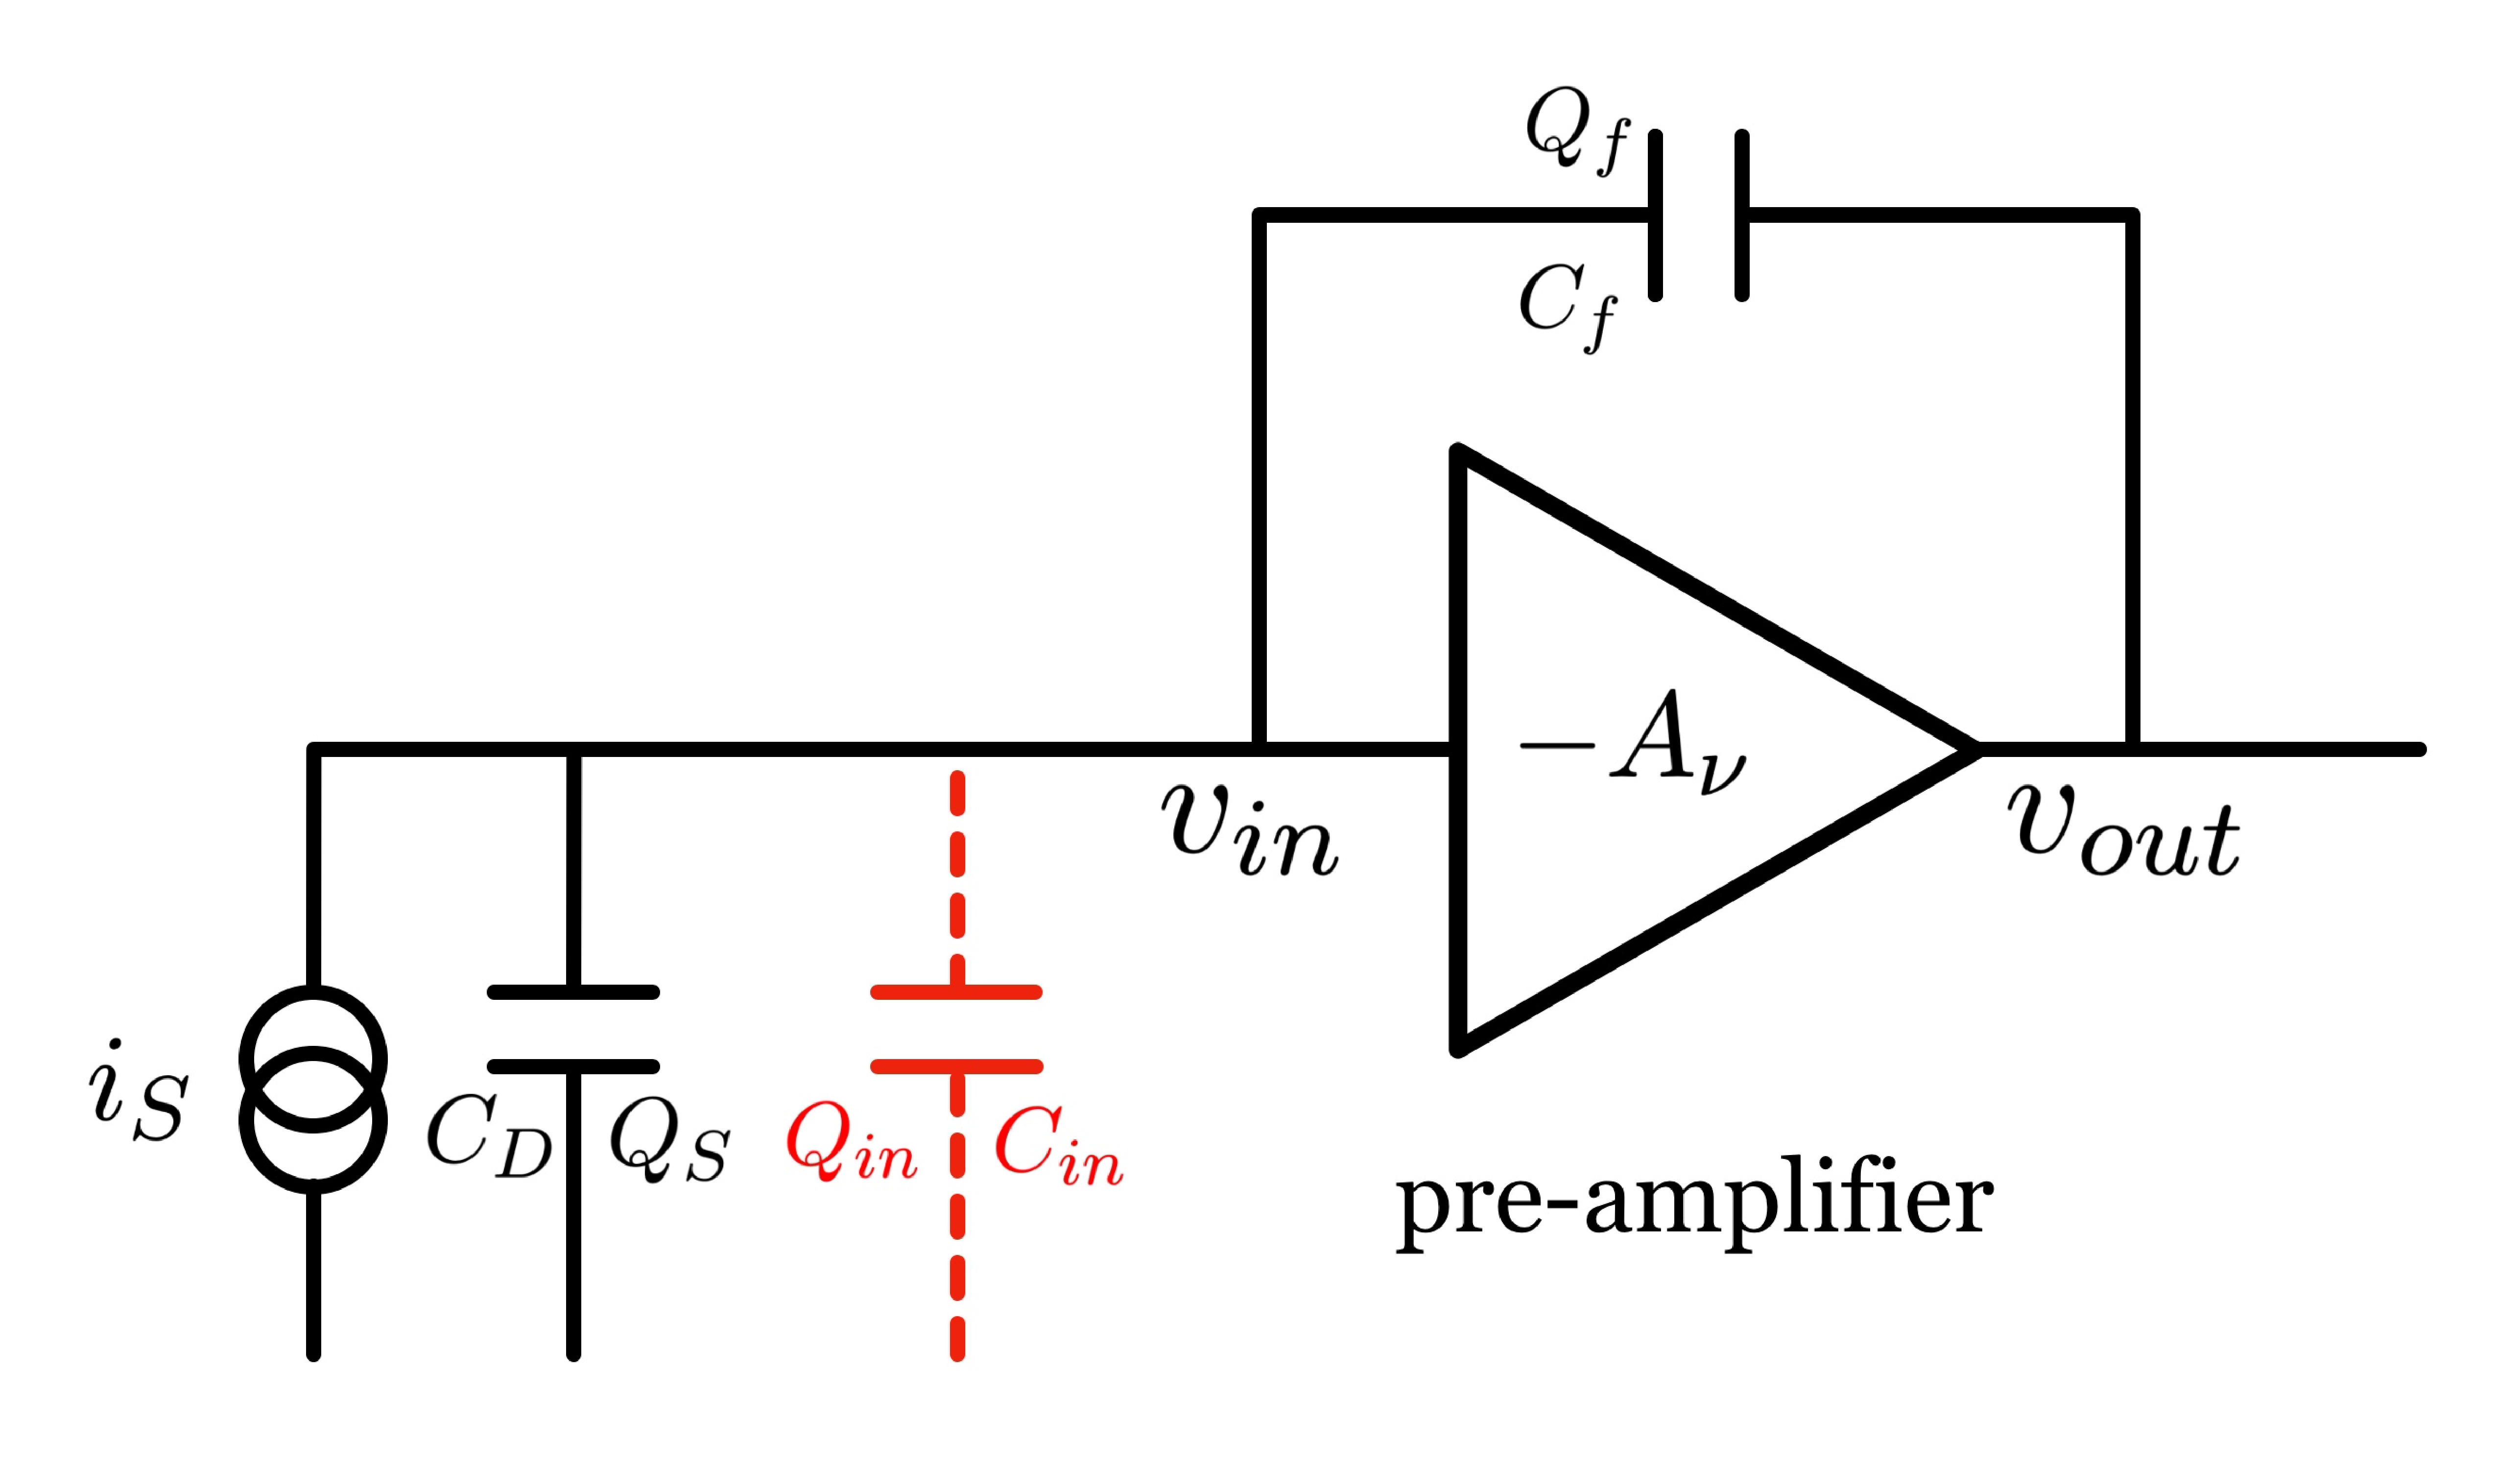
\includegraphics[width=0.9\linewidth]{files/CSA_block_diagram}
		\caption{Charge Sensitive Amplifier block diagram}
		\label{ }
		\end{minipage}
		\end{figure*} 

		The output voltage of the inverting OpAmp can be written as a function of the feedback capacity $C_f$ as follows: 
		\begin{equation}
			v_{out}(t) = -A_\nu v_{in}(t) = -\frac{1}{C_f} \int_0^t i_S(t') dt' = -\frac{Q_{in}(t)}{C_f}
		\end{equation}
		The voltage difference over the feedback capacitor is given by: 
		\begin{equation}
			v_f = v_{in} - v_{out} = v_{in}(1+A_\nu) = \frac{Q_f}{C_f}
		\end{equation}
		Since there is no current flowing into the OpAmp, the feedback charge $Q_f$ on the capacitor $C_f$ is equal to the signal charge in input to the amplifier $Q_{in}$. One can then define a dynamic input capacitance for the amplifier: 
		\begin{equation}
			C_{in} = \frac{Q_{in}}{v_{in}} = C_F(1+A_\nu)
		\end{equation}
		For sufficiently large internal gain of the OpAmp, the charge amplification can be characterised by its charge gain and reads: 
		\begin{equation}
			A_Q = \frac{v_{out}}{Q_{in}} = \frac{-A_\nu v_{in}}{(C_{in}v_{in})} \approx \frac{-A_\nu}{1+A_\nu} \frac{1}{C_f} \approx -\frac{1}{C_f}
		\end{equation}
		
		In practice, the capacitance of the detector is not negligible, and some charge remains in the detector since it is partitioned between the detector capacitance and the amplifier's feedback capacitance. The ratio between the charge in input to the amplifier and the total induced charge $Q_S$ is given by:
		\begin{equation}
			\frac{Q_{in}}{Q_S} = \frac{C_{in}}{C_{in} + C_D} = \frac{1}{1+\frac{C_D}{(1+A_\nu)C_f}}
		\end{equation}

		It is interesting so see that the gain of a CSA depends on the feedback capacitance. This is an important aspect as one can understand that if the feedback capacitance would be a free parameter of the front-end, one could act on the sensitivity to input charge desired for a (nearly) constant discrimination threshold in the discriminator. Although, for high gain of the amplifier, i.e. low feedback capacity $C_f$, if the detector capacity is significantly larger, a non-negligible part of the charge will remain in the detector. The charge gain of the amplifier can be corrected accordingly so that: 
		\begin{equation}
			A_Q = \frac{v_{out}}{Q_S} = \frac{v_{out}}{Q_{in}}\frac{Q_{in}}{Q_S} = \frac{-A_\nu}{1+A_\nu} \frac{1}{C_f} \cdot \frac{1}{1+\frac{C_D}{(1+A_\nu)C_f}} \approx - \frac{1}{C_D + \frac{C_f}{A_\nu}}
		\end{equation} 
		Even in the case, a large voltage gain $A_\nu \gg C_D/C_f$ is going to give the same result as before where the charge gain only depends on the inverse of the feedback loop capacitance. These considerations are made for an ideal case of an amplifier with infinitely large bandwidth (BW) or equivalently infinite input impedance $Z_{in}$. 

		This condition is not necessary realised for BJTs but if we denote by $R_{in}$ the input resistance of the amplifier, the above discussion holds if the following condition on the input impedance is realised:
		\begin{equation}
			Z_{in} \gg \frac{1}{2 \pi f_P C_{in}} \hspace{5mm} \Rightarrow \hspace{5mm} f_P \gg \frac{1}{2\pi Z_{in} {\left( 1 + A_\nu \right)C_f}}
		\end{equation}
		The above equation show the condition under which the transfer function of the amplifier becomes that of a typical integration circuit. For the BJT this translates to the fact that the impedance associated to the feedback capacity $C_f$ is small enough compared to $R_{in}$ so that all the current flows to the feedback loop made by the feedback resistance and the capacitance between the base and the collector of the BJT. Unless the amplifier is operated at frequencies higher than the first pole of the amplifier, in a region where the ratio between input and output exhibit a - \SI{20}{\decibel}/decade slope, it won't behave as a CSA. The finite BW will also put a constraint on how fast the output voltage can rise but will also provide more stability to the amplifier as it means operating it at lower gain. A comparison between ideal and realistic response in the frequency and time domain are presented in the figure below:  
		
		\begin{figure}[h]
		\centering
		
\includegraphics[width=0.9\linewidth]{files/CSA_transfer_function}
		\caption{Transfer function of a Charge Sensitive Amplifier}
		\label{ }
		\end{figure}
		\note{Put the diagram with impedance and not $A_v$ on the axis vertical axis}
		\note{Should I insert a schematic view of the front end with the BJT ?}\\
		In the ideal case of a CSA discussed previously, theew is no resistor in the feedback loop but only the feedback capacitor, this leads to an output level constantly increasing with time for every signal inputed in the amplifier. The addition of the feedback resistance plays a role in discharging with exponential characteristics the feedback capacitance in the feedback loop with a time constant given by $\tau_{discharge} \simeq R_f {\left( C_{det} + C_f (1+A_\nu) \right)}$ \note{add value for our BJT}. The discharge time is an essential parameter of the front-end electronics as it also contributes in defining was is the maximal rate at which the detector can be operated. The same resistance is also essential for controlling what is the voltage gain of the amplifier as it controls how much current from the output is re-injected in the input. As seen in \note{insert figure ref}, since the amplifier inverts the input signal, by reducing the feedback resistance, the voltage gain is reduced as more signal of opposite polarity is injected in the input.
		
		
		\subsection{Equivalent Noise Charge}\label{subsec:2.3.3}
		Since there exist no perfectly accurate measurement system, the characterisation of the noise contribution to the total signal noise is essential in defining both the timing performance and the energy or charge sensitivity of a detector coupled to a readout system. The influence on the noise on the signal from the detector is mainly associated in semiconductors to Landau fluctuations in the charge deposition across the detector's thickness as well as recombination of electron hole pairs. Fortunately, the contribution to the noise from the detector is negligible in contrast to the electronic noise \cite{detectors}. Recalling that a detector readout system implements a discriminator stage comparing the output of the amplifier to a threshold voltage, it becomes clear that the lower the voltage noise and the more sensitive the detector will be to small energy deposition. Concerning the timing performance of the detector system, the time resolution $\sigma_t$ has various contributions both from different aspects of the front-end discussed later (\note{cite the section}) but is often limited by the time jitter ($\sigma_{jitter}$) defined as follows: 
		\begin{equation}
			\sigma_{jitter} = \frac{\sigma_V}{\frac{dV}{dt}}\simeq  \frac{t_{rise}}{SNR} = \frac{\sigma_V}{A_q} \frac{t_{rise}}{Q_{in}} \hspace{4mm} \rightarrow \hspace{4mm} \sigma_{jitter} = \frac{ENC}{i_{S}}
			\label{eq:time_jitter}
		\end{equation}
		where we have introduced $\sigma_V$ as the voltage noise on the signal, $dV/dt$ the signal's slope, $t_{rise}$ the rise time of the signal and $SNR$ the Signal to Noise Ratio of the front-end defined as the ratio of input charge scale to the charge gained by the signal's voltage noise. The last step in equation \eqref{eq:time_jitter} introduced the concept of Equivalent Noise Charge (ENC) and represents the input charge in electrons that would need to be fed to the input of the amplifier in order to produce an output voltage equivalent $\sigma_V$. Noise is usually the consequence of fluctuations, in this case of charge carrier densities $N$ or velocities $v$ so that the fluctuation on a current flowing between two electrodes separated by a distance $d$ can be expressed as: 
		\begin{equation}
			i = \frac{Nev}{d} \hspace{5mm} \rightarrow \hspace{5mm} \sigma_i^2 = {\left( \frac{ev}{d} \sigma_N \right)}^2 + {\left( \frac{eN}{d} \sigma_v \right)}^2
		\end{equation}
		Three different noise sources can be identified: the thermal noise associated to the thermal fluctuation in velocities of charge carries, the shot noise and $1/f$ noise which are collectively associated to the variation in number density of charge carriers \cite{detectors}.
		For a BJT, two separate equivalent noise sources can be identified that are the parallel and series noise sources. The first noise source accounts for thermal noise in the base resistance of the BJT and shot noise in the collector while the more significant parallel noise accounts for shot noise produced by the leakage current in the base. The contribution to the ENC from the amplifier can be qualitatively expressed as a function of the shaping time $\tau_m$ such that:    
		\begin{equation}
  			ENC(\tau_m) = \sqrt{2 \frac{a}{\tau_m} {\left( C_{det} + C_{in} \right)}^2 + 4 \frac{\ln(2)}{\pi} b{\left( C_{det} + C_{in} \right)}^2 + \frac{2}{3}c \tau_m} 
		\end{equation}
		where $a$, $b$ and$c$ respectively accounts for the series white noise sources, $1/f$ noise which is usually negligible for BJTs \cite{Paolozzi_thesis} and parallel white noise sources. This expression shows that for integration of fast signals, the contribution of the BJT to the ENC will be dominated by the series noise while at higher integration times ( \SI{1}{\micro\second} and above), the parallel noise takes over and the leakage current of the base of the transistors deteriorates its desired low noise performance. Looking more in detail into the series noise of the BJT, it can be qualitatively expressed as a function of the base resistance $R_b$ and the current gain $\beta$ and reads \cite{Paolozzi_thesis}: 
		\begin{equation}
  			ENC_{series \hspace{1mm} noise} \propto \sqrt{k_1 \frac{{\left( C_{det} + C_{in} \right)}^2}{\beta} + k_2 R_b {\left( C_{det} + C_{in} \right)}^2}
  			\label{eq:ENC_series}
		\end{equation}
		where $k_1$ and $k_2$ are constants. The above equation shows that in order to further mitigate the contribution of the series noise in a BJT, one would need to have a reduced the base resistance $R_b$ and also profit from a high current gain $\beta$. 

		
		\subsection{SiGe BiCMOS HBTs}\label{subsec:2.3.4}
		
		The SiGe BiCMOS technology implements into standard CMOS nodes a SiGe HBT and is used in diverse field where low noise and very fast amplifiers are required. In regular silicon BJTs amplifiers, the transport mechanism of charges in the base is governed by diffusion which is a relatively slow and inefficient process due to its isotropic nature. A faster and much more efficient transport mechanism is drift, which requires the presence of an electric field driving the movement of charges toward the collector. The introduction of an epitaxially grown SiGe film in the base of the transistor with a linearly graded Germanium profile produces the band structure as follows. 
		\begin{figure}[h]
		\centering
		\includegraphics[width=0.9\linewidth]{files/SiGeBand_Structure}
		\caption{Band structure of a BJT (dashed line) in comparison to the ones of a SiGe HBT (solid line) \cite{SiGEHBT_band_Structure}}
		\label{im:SiGe_bandstructure}
		\end{figure}
		
		The band structure of such a device effectively implements an electric field driving the drift mechanism of electrons from the base of the transistor into the collector. The net effect is an increased current gain $\beta$ resulting in an improved transition frequency $f_T$. A secondary benefit of the SiGe HBTs comes from the directionality of the transport mechanism. In standard BJT, in order to maximise charge injection efficiency, a large collector-base surface contact is needed but this is no longer the case for SiGe HBTs. The size of the collector-base contact can be reduced hence reducing the collector base capacitance $C_{BC}$. As discussed in section \subsecref{subsec:2.3.2}, the gain of the amplifier is proportional to the inverse of the capacitance in the feedback loop which is for the BJT the collector-base capacitance, this effect also lead to a much higher charge amplification. Finally the smaller size of the base also reduces its resistance $R_b$ giving the SiGe HBTs, along with the high current gain $\beta$, the two key features required to minimise the ENC of the BJT and enhance its low noise performances.
		
		The 130nm SiGe BiCMOS HBT node from IHP (SG13G2) can reach a cut-off frequency of $f_T = $ \SI{350}{ \giga\hertz} when alimented with the nominal bias, for this reason and all the advantages discussed previously, this technology was used in the different ASICs studied in this work, It is important to specify that SiGe HBTs were implemented only in the regions requiring high analog performance where as the rest of the design (98\%) used standard CMOS technology \cite{Picardi_thesis}. When operating such amplifiers, what defines the working point of the device is the desired gain in a range of operating frequencies. By increasing the bias given to the amplifier, the cut-off frequency increases, increasing at fixed gain the bandwidth and allowing a higher operation frequency. On the contrary if the power consumption of the device is a constraint, reducing the bias given to the amplifier with reduce its bandwidth. 
		
		Throughout this work, both type of operations will be discussed, for very different applications. The MONOLITH project aims at developing an ASIC for ultra fast timing and so will require operating the transistor in the high transition frequency regime as discussed in \note{insert ref to section about monolith ASICs} whereas the ASIC designed for FASER has stricter requirements on power consumption than timing performance which will be discussed in details in \note{insert reference to section discussing FASER ASIC requirements}.   
		
		
		\clearpage

	\section{Pixelated detector technologies }\label{sec:2.4}
	
	Semiconductor devices in High Energy Physics (HEP) are usually arranged in two different geometries. Strip detectors which consist of long and fine collection electrodes with a pitch in the range of \SI{50}{\micro\meter} to \SI{100}{\micro\meter}. Pixelated detectors implementation, which we will focus on throughout this discussion, are subdivided in multiple sensitive areas arranged in a periodic pattern, like an additional subdivision of the strip. The pixel defines the smallest sensing unit in the detector and the position information of the passage of the particle is associated to the position of the pixel in the detector. If we define as $p$ the pitch on a specific direction of the pixelated detector (as pixel do not necessarily have a the same pitch in every space dimension), and $\rho(x)$ the probability density function, the resolution on the hit position of the particle is defined as follows: 
	\begin{equation}
		\sigma_x^2 = \int_{-p/2}^{p/2} x^2 \rho(x) dx = \frac{1}{12} p^2 \hspace{4mm} \rightarrow \hspace{4mm} \sigma_x = \frac{1}{\sqrt{12}} p
		\label{eq:spatial_resolution}
	\end{equation} 
	The above equation is valid for squared and rectangular pixels, for more specific geometries like hexagonal pixels used in this work, one need to build the probability density function along one of the axis used for the reference system using hexagonal pixel and compute the integral as in \eqref{eq:spatial_resolution} and would obtain $\sigma = \sqrt{\frac{5}{24}}p$. The resolution is the same along any axis of the hexagon. \\ \note{cite Matteo's Thesis}

	When an electronic readout systems needs to be coupled to the active part of the detector, two approaches are usually considered: 
	\begin{itemize}
		\item Hybrid detectors, for which the sensitive part of the detector and the readout system are implemented in two different dies and are later interconnected during the assemble procedure,
		\item Monolithic detectors, implementing directly within the same silicon die, both the sensitive part and the readout electronics. 
	\end{itemize}
		Both implementation technologies have advantages and limitations and a non exhaustive comparison between the two will be presented in the following subsections. 
	
		\subsection{Hybrid pixel detectors }\label{subsec:2.4.1}
	
		Hybrid pixelated detectors are assembled devices where the active chip is manufactured is a sensor grade silicon substrate while the readout chip is manufactured in a different silicon substrate more suited for the integration of readout electronics. Both chips have a pixelated electrode structure and are required to have a precise match between the two chips for both pixel pitch and electrode size so that each pixel on the sensitive chip has a one to one geometrical correspondence to a pixel on the readout chip.
		
		\note{could substitute sensitive chip with active and readout chip with passive}
		The connection between the two electrode on each chips is realised with a conducting micro-connection also called bump bond, which consists in the creation through diverse techniques of a soldering metallic ball directly on top of the electrodes of the readout chip \cite{flipChip}. The two chips are then put together using state of the art flip-chip techniques, precisely aligning the two dies and soldering the electrodes together through the soldering ball. Historically, bump bonding techniques were considered as a bottleneck for achieving high pixel density devices with typical sizes of \SI{150}{\micro\meter} \cite{flipChip}. Thanks to the technical improvements in the bump deposition process, the connection can now be relatively short, usually in the range of \SI{10}{\micro\meter} to \SI{20}{\micro\meter} allowing for very dense designs and mitigating unwanted parasitic effects. 
		
		\begin{figure}[h]
			\centering
			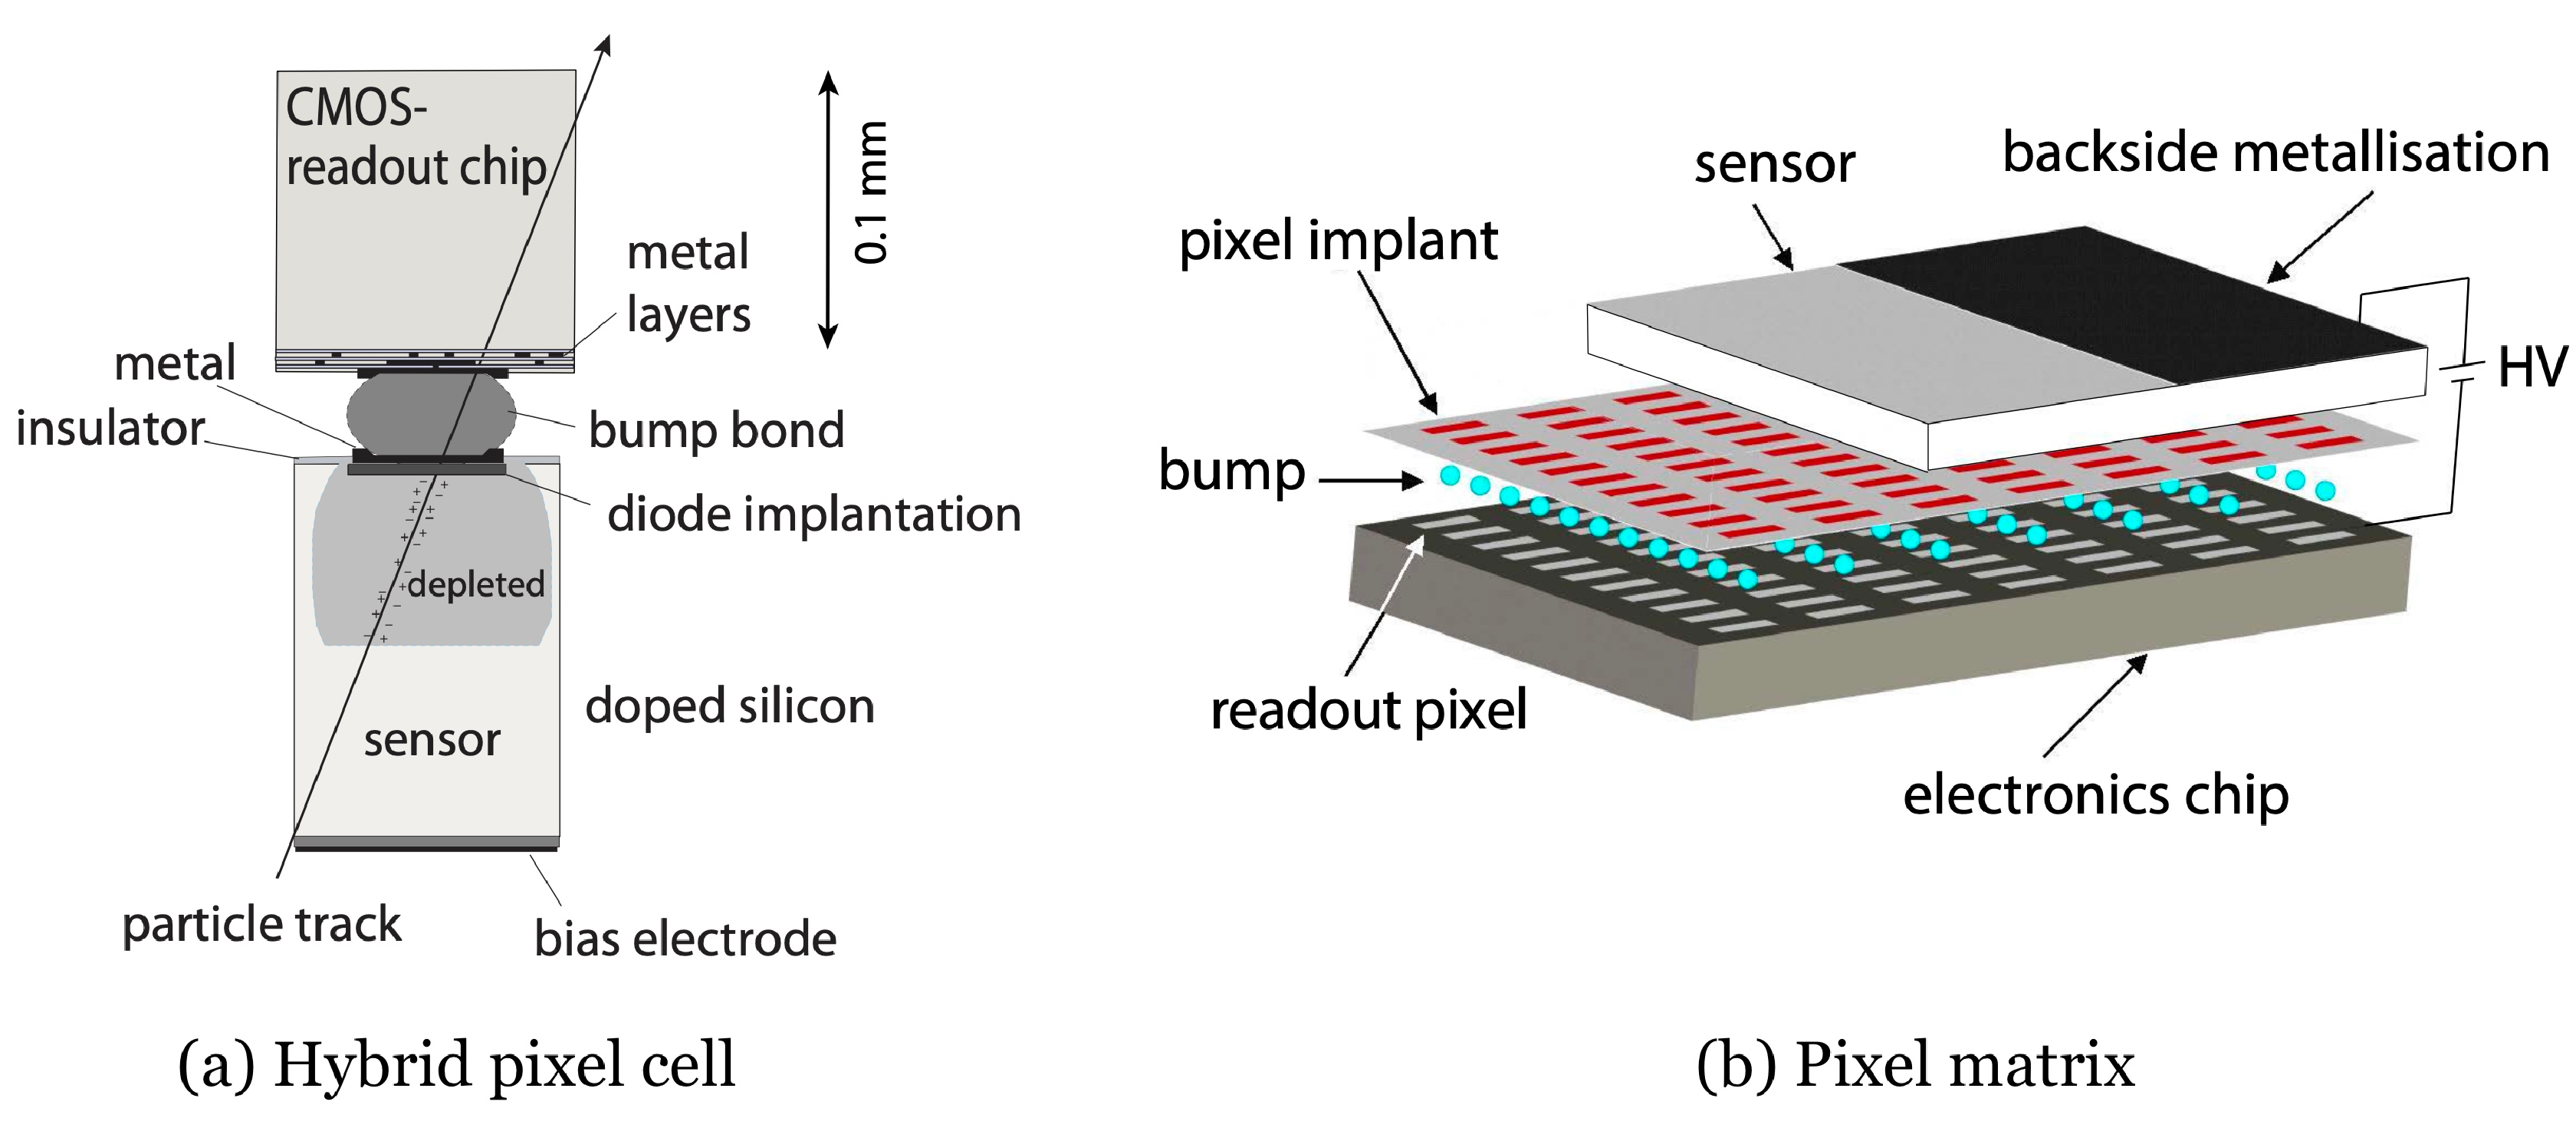
\includegraphics[width=0.9\linewidth]{files/hybrid_detector}
			\caption{Hybrid pixel detector: (a) layout of an individual pixel cell with both active (bottom) and passive (top) parts and (b) matrix of pixels showing the pixelisation of both the active sensor and readout electronics sensor, interconnected through bump-bonding \cite{detectors}}
			\label{ }
		\end{figure}
		
		 The sensitive chip often consists in pixels of \SI{50}{\micro\meter} pitch to enhance spatial resolution and have a sensor thickness typically in the range of \SI{300}{\micro\meter}. The capacitance of these devices is usually in the range of \SI{100}{\femto\farad}, mostly affected by the neighbouring pixels rather than the backside due to their thickness. As mentioned before, the detector capacitance plays a key role in defining the performance of the sensor once coupled to readout electronics. Typical hybrid sensors provide timing performances in the order of \SI{10}{\nano\second} and their low noise and low power consumption has made them suitable candidates for many HEP applications \cite{Picardi_thesis}. 
		 Many LHC experiments have chosen hybrid devices to build the inner-most tracker of their detector \cite{pixel_vertex_detector}. This region being very close to the collision point, it is exposed to a very harsh radiation environment with fluencies reaching after 10 years of operation levels of $10^{15} $ 1 MeV neutron equivalent/ cm$^2$. The detectors chosen for these inner trackers implement planar silicon sensors for the sensitive chip and have proven to be radiation tolerant and remain operable in their operation time scales. 
		 
		 The architecture of hybrid pixelated detectors makes possible a separate but parallel development and improvment of the sensitive and the readout chip in order to achieve better performances. For applications concerned with fast timing performances, readout chips like the TimePix4 \cite{timepix4} ASIC have already demonstrated a time resolution of \SI{60}{\pico\second} and some more ambitious projects like PicoPix \cite{picoPix} aims at a time resolution of \SI{10}{\pico\second}. This time resolution is only a constituent of the bigger picture where the intrinsic time resolution of the sensitive chip needs to be accounted for too. Nowadays the most promising technologies are 3D trenches silicon sensors for reduced charge collection time and planar silicon sensors with gain layer for internal charge amplification and reduced electronic noise.  \\
		 
		 Hybrid pixelated detectors have demonstrated their ability in providing a solution in terms of detector compactness, spatial and timing resolution needed for the very constrained and highly performance-demanding region that is the one closest to the interaction point in HEP experiments. Nevertheless this detector technology still present as of today some limitations like their complex and expensive manufacturing and assembly procedure. The material cost is improved in contrast to older detector technologies but the need for a sensitive chip, readout chip, support and cooling still constitutes a restrain for further improvements in overall detector performance. 
		  
		
		\subsection{Monolithic pixel detectors }\label{subsec:2.4.2}
		
		Pixel detectors made their way to particle physics experiments in the beginning of 1990 and soon started to fill the detectors of the LHC experiments. In parallel to the development of hybrid pixelated detectors, some efforts were made to develop monolithic, but were first discarded as the progress made in performance with hybrid implementation made them suitable candidates for various applications \cite{pixel_wheredowestand}. After a bit of time, improvements in the maximum resistivity of the substrate for the operation of the electronics but also in the size of the transistors used in the electronics themselves made monolithic pixel detectors more attractive. They indeed not only reached the level of performance required to make them attractive for LHC experiments but also put forward compelling advantages with respect to hybrid implementation. \\
		
		Monolithic pixelated detectors have both the sensitive part of the detector and its readout electronics included in the same substrate making it a single entity. This unlocked the potential to produce a full detector system using standard CMOS process \cite{Picardi_thesis}. 
		
		The first advantage of a monolithic implementation has already been put under light: the complex and costly assembly process of hybrid detectors is no longer an issue and allows the production of low-cost and large volumes together brought up by the use of CMOS technology. For LHC experiments applications, the material cost is an essential factor as it influences the resolution on the reconstructed track associated to a particle, more material increases multiple scattering and reduces the resolution. For the ATLAS and CMS experiments, the hybrid pixel detector represent a material thickness in excess of 3$\%$ of a radiation length per detector layer \cite{detectors}. The active sensor and passive readout electronics being in a the same substrate for monolithic pixel detectors, the material cost could be reduced up to a factor of magnitude if the detector can be build on a self-supporting structure and operated with low enough power densities to minimise the need for cooling \cite{detectors}. The requirements on monolithic pixel detectors also include a sufficiently large signal-to-noise ratio to allow for a low noise operation together with a good radiation tolerance against ionising and non-ionising radiation (for more details on radiation tolerance see \note{cite section}). 
		
		The ability to use the full CMOS technology, meaning both NMOS and PMOS transistor on the same substrate is essential to unlock the true potential of CMOS logic in monolithic detectors. Initially monolithic sensors were made using a low resistivity p-type substrate on which an epitaxial Silicon layer was grown with higher resistivity than the substrate and freedom in the choice of type. A schematic view of such a sensor is given in the figure below: 
		\begin{figure}[h]
			\centering
			\includegraphics[width=0.9\linewidth]{files/MAPS_noHV}
			\caption{Cross section view of a typical monolithic sensor implementation without external bias voltage for depletion and including both PMOS and NMOS transistors.}
			\label{im:initial_mono_XS}
		\end{figure}
		
		 The thickness of the epi-layer depends on the applications and is usually in the 1-\SI{20}{\micro\meter} range, the electronics are then implanted at the top of the epi-layer. When particles cross the epi-layer, charge can be deposited both in the small depleted region below the collection electrode and mainly in the non depleted epi-layer. The collection of charge from the depleted region will be fast and complete thanks to the drift of charges carriers whereas the collection from charges from the non depleted epi-layer will be driven by diffusion and hence be incomplete and comparatively slow ($>$ \SI{100}{\nano\second}) \cite{detectors}. The collection electrode is in this case a n-type well and the use of NMOS transistors laying in a p-type well is not problematic whereas the use of PMOS transistors laying in a n-type well would constitute a competing electrode for charge collection. For this reason, n-type well for electronics have to be shielded by a deep highly doped p-type well implanted below the n-type well in the epi-layer. 
		 
		 This design offers as an advantage a reduced total thickness (in contrat to hybrid detectors) in the range of 50-\SI{150}{\micro\meter} \cite{detectors} and hence a reduced material cost per layer  if implemented in an experiment. The down-side is the time resolution of such devices, which would only be suitable for experiments such as the ALICE detector for heavy ions collisions \cite{alpide}. In order to obtain a much faster and complete charge collection to satisfy requirements or other LHC experiments, it is straightforward that monolithic sensors have to be fully depleted to have a drift-driven charge transport in the active part of the sensor. As seen in equation \eqref{eq:depletion_width}, the depletion thickness can be written such as: 
		 \begin{equation}
		 	d_{depletion} \approx \sqrt{V \rho}
		 \end{equation}
		
		This implies that the choice of process technologies employed must allow higher voltages than the ones usually required by standard CMOS technologies \cite{peric} or be able to process high resistivity wafers, or a combination of both \cite{detectors}. The chosen technology also needs to provide multiple wells both for shielding and implementation and NMOS and PMOS transistors. Two different approches in realising such detectors have been considered: the small collection electrode and large collection electrode design which we will now discuss.
		
		\subsubsection{Small Collection Electrode}
		The small electrode configuration has a n-type well separated from the CMOS electronics, due to its shrunk size it allows for a small collection node capacitance in the range of 5-\SI{20}{\micro\meter} \cite{detectors} which is of concern for noise and timing performances as seen in \eqref{eq:ENC_series} and \eqref{eq:time_jitter}. This implementation is also not optimal in terms of radiation tolerance as trapping probability of defects in the lattice (see more in \note{cite section on rad tolerance}) is linked to the collection time and is usually longer for small electrodes as the electric field is not uniform across the region separating two electrodes. The figure below gives a generalised schematic view of the small collection electrode implementation: 
		\begin{figure}[h]
			\centering
			\includegraphics[width=0.9\linewidth]{files/MAPS_small_electrode}
			\caption{Schematic cross section of the small electrode implementation for monolithic pixel sensors. An additional n-type layer is added to ease the full depletion of the sensor.}
			\label{im:small_electrode}
		\end{figure}
		
		Achieving full depletion in small electrodes designs is not straightforward and a modification of the process involving the addition of a low dose n-type implant below the pixel is required \cite{thanu_small_electrode}. This modification has the overall effect of strengthening the electric field laterally and so improve charge collection laterally too. The small charge signal created in the thin epi-layer (typically in the range of 1600 $e^-$)\cite{detectors} is not too much of a constraint as the collection node capacitance is small and since the voltage is given by $dv = dQ/C_D$, resulting in a voltage difference in the range of \SI{50}{\milli\volt}, a voltage amplification stage is hence usually used. 
		For small electrodes design, a small pixel size is usually preferred to mitigate the negative effect on radiation tolerance and timing performance, this comes at the cost of a higher required power density as the power consumption is roughly constant per pixel. 
		
		
		\subsubsection{Large Collection Electrode}
		The alternative is a large collection electrodes for the implementation of monolithic pixels detectors. This means that the collection electrodes covers most of the area of the pixel, this leads to a set of advantages but also limitations in contrast to the small collection electrode. The figure below presents a generalised schematic view of the large collection electrode implementation. 
		\begin{figure}[h]
			\centering
			\includegraphics[width=0.9\linewidth]{files/MAPS_large_electrode}
			\caption{Schematic cross section of the large collection electrode implementation for monolithic pixel detectors.}
			\label{im:large_collection_electrode}
		\end{figure} 
		
		In this configuration, full depletion is achieved from the top surface or from the backside through the realisation of a backside processing allowing for a backside contact for depletion voltage.
		Having a much more uniform weighting field, the collection of charges is more uniform and also faster as the collection path is shorter than for small collection electrodes. This benefits to the radiation tolerance of the sensors since the trapping probability will be reduced, but also to the timing performance. On the contrary, the large collection electrodes, together with the implementation of close-by deep n-type and p-type wells, presents to the input of the amplifier a large detector capacitance (in the range of several hundreds of \SI{}{\femto\farad}), having a negative impact on both noise and timing performances. An optimisation of both electrode geometry and internal junctions is essential to a reach the best performances of the sensor for a fixed power consumption \cite{Picardi_thesis}. \\
		
		Many different pixel designs have been realised in both configurations, showing a high rate capability and radiation tolerance to comply with the level required at the LHC \cite{detectors}. Throughout this work, monolithic pixel detectors with large collection electrodes will be presented. This work will not focus on the design of such devices but rather on the extensive qualification and understanding of their features, both for the development of the FASER Pre-Shower but also for the ultra fast timing performances of concern for the MONOLITH project. 
		\clearpage

	\section{Effects of radiation \textcolor{blue}{ 4 pages}}\label{sec:2.6}
		\subsection{Processes involved \textcolor{red}{ 2 pages}}\label{subsec:2.6.1}
		\subsection{Consequences of damages and solutions \textcolor{red}{ 2 pages}}\label{subsec:2.6.2}
